\begin{apendicesenv}

\partapendices
\chapter{Protótipo}
\label{apendice:prototipo}

Tendo como base todo o processo de Lean Inception feito durante o desenvolvimento deste trabalho, realizou-se o desenvolvimento do protótipo de alta fidelidade. A partir desse protótipo, desenvolveu-se as figuras~\ref{p1} a~\ref{p18}, que representam uma visão fiél de como as telas se comportariam em um celular Android.

\begin{figure}[H]
    \centering
    \caption{Tela de Flashcards sem Cards.}
    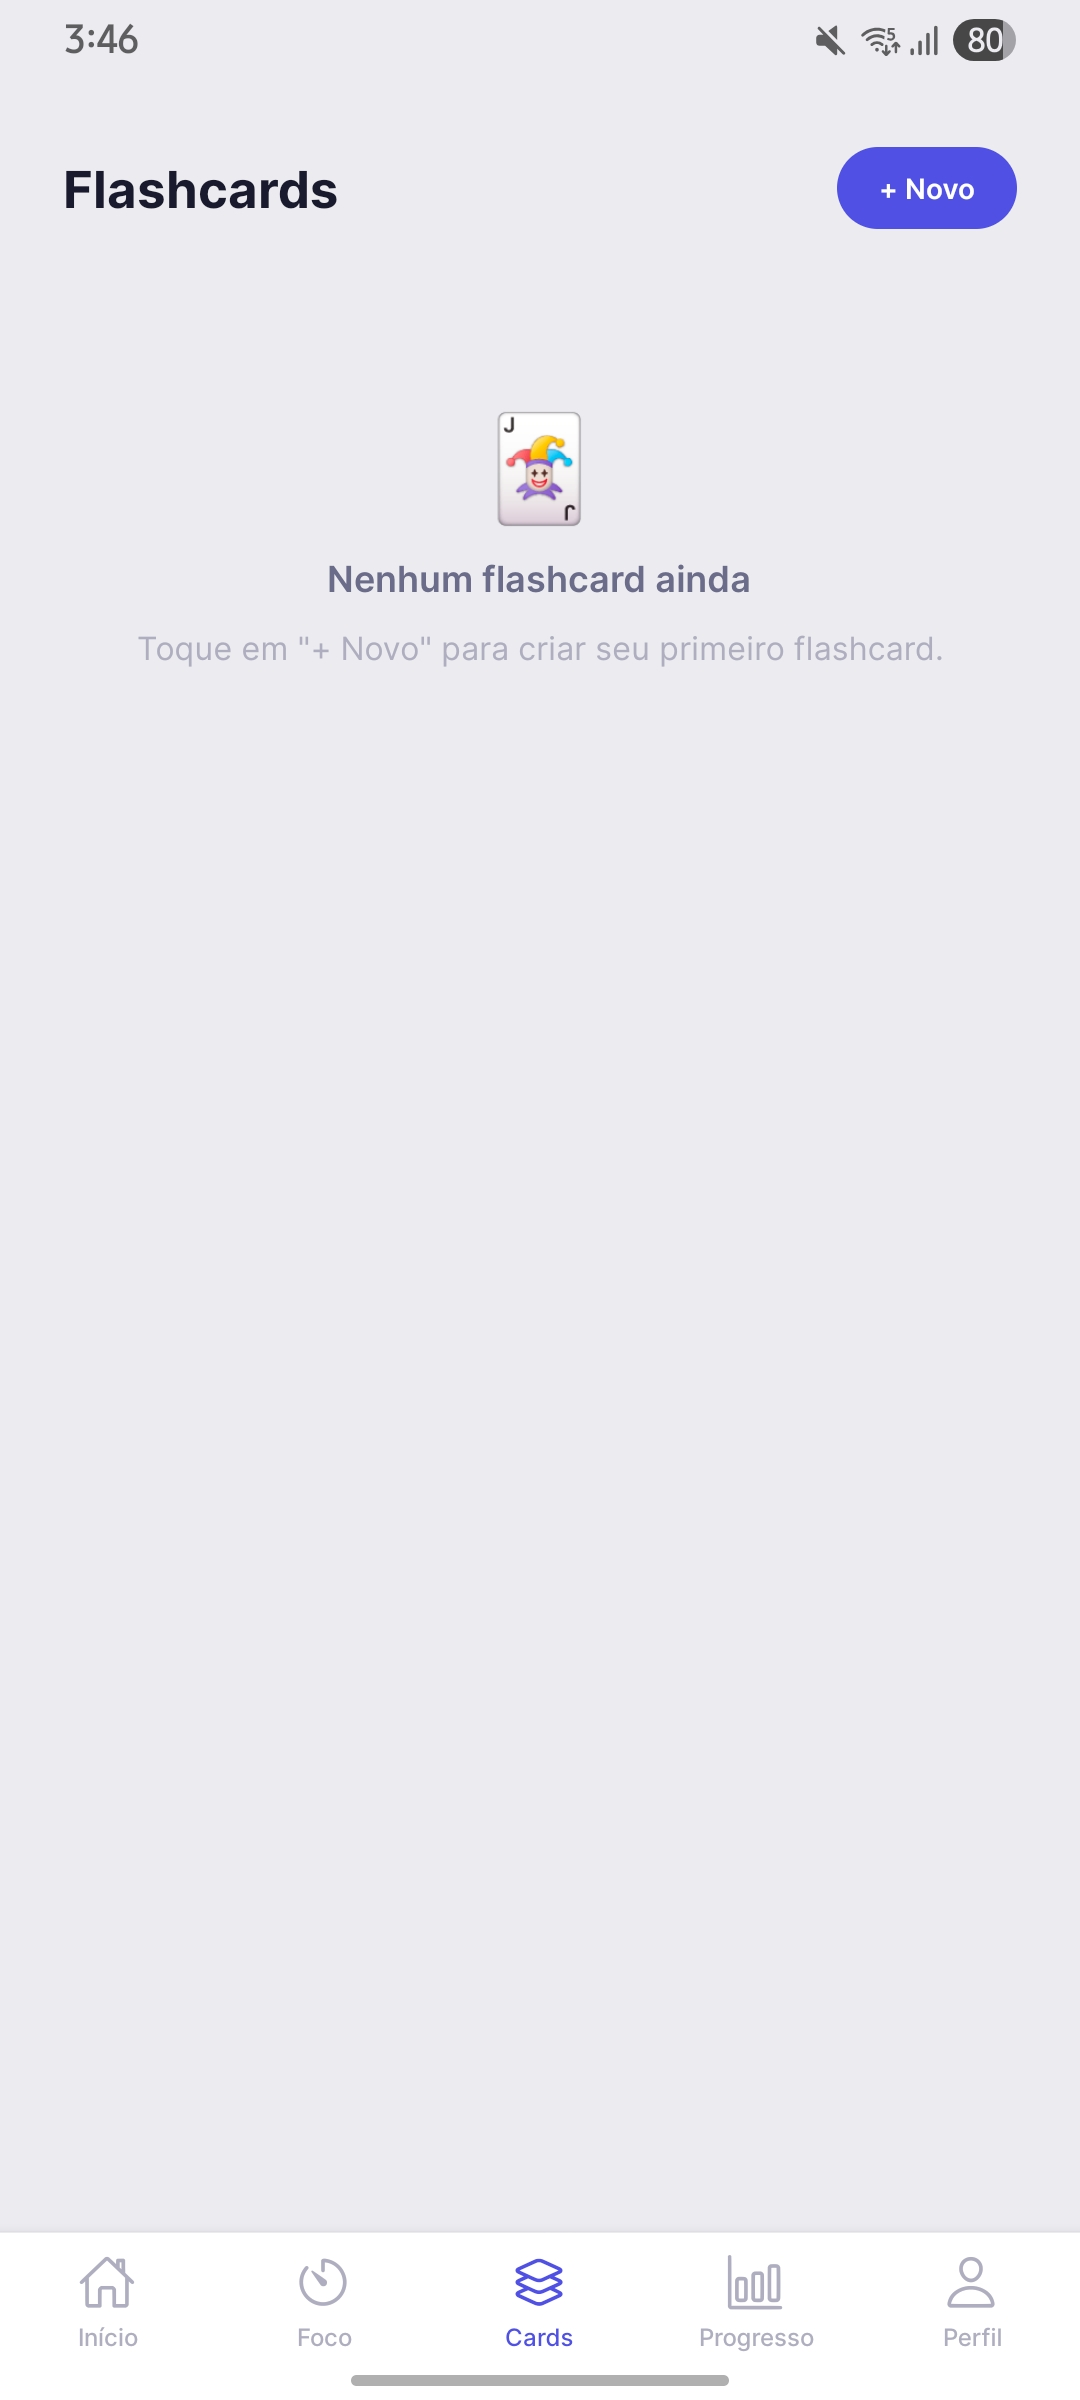
\includegraphics[height=0.7\textheight]{Imagens/PrototipoFigma/00_flashcards_empty.jpg}
    \par
    Fonte: autoria própria.
    \par
    \label{p1}
\end{figure}

\begin{figure}[H]
    \centering
    \caption{Tela de Onboarding 1.}
    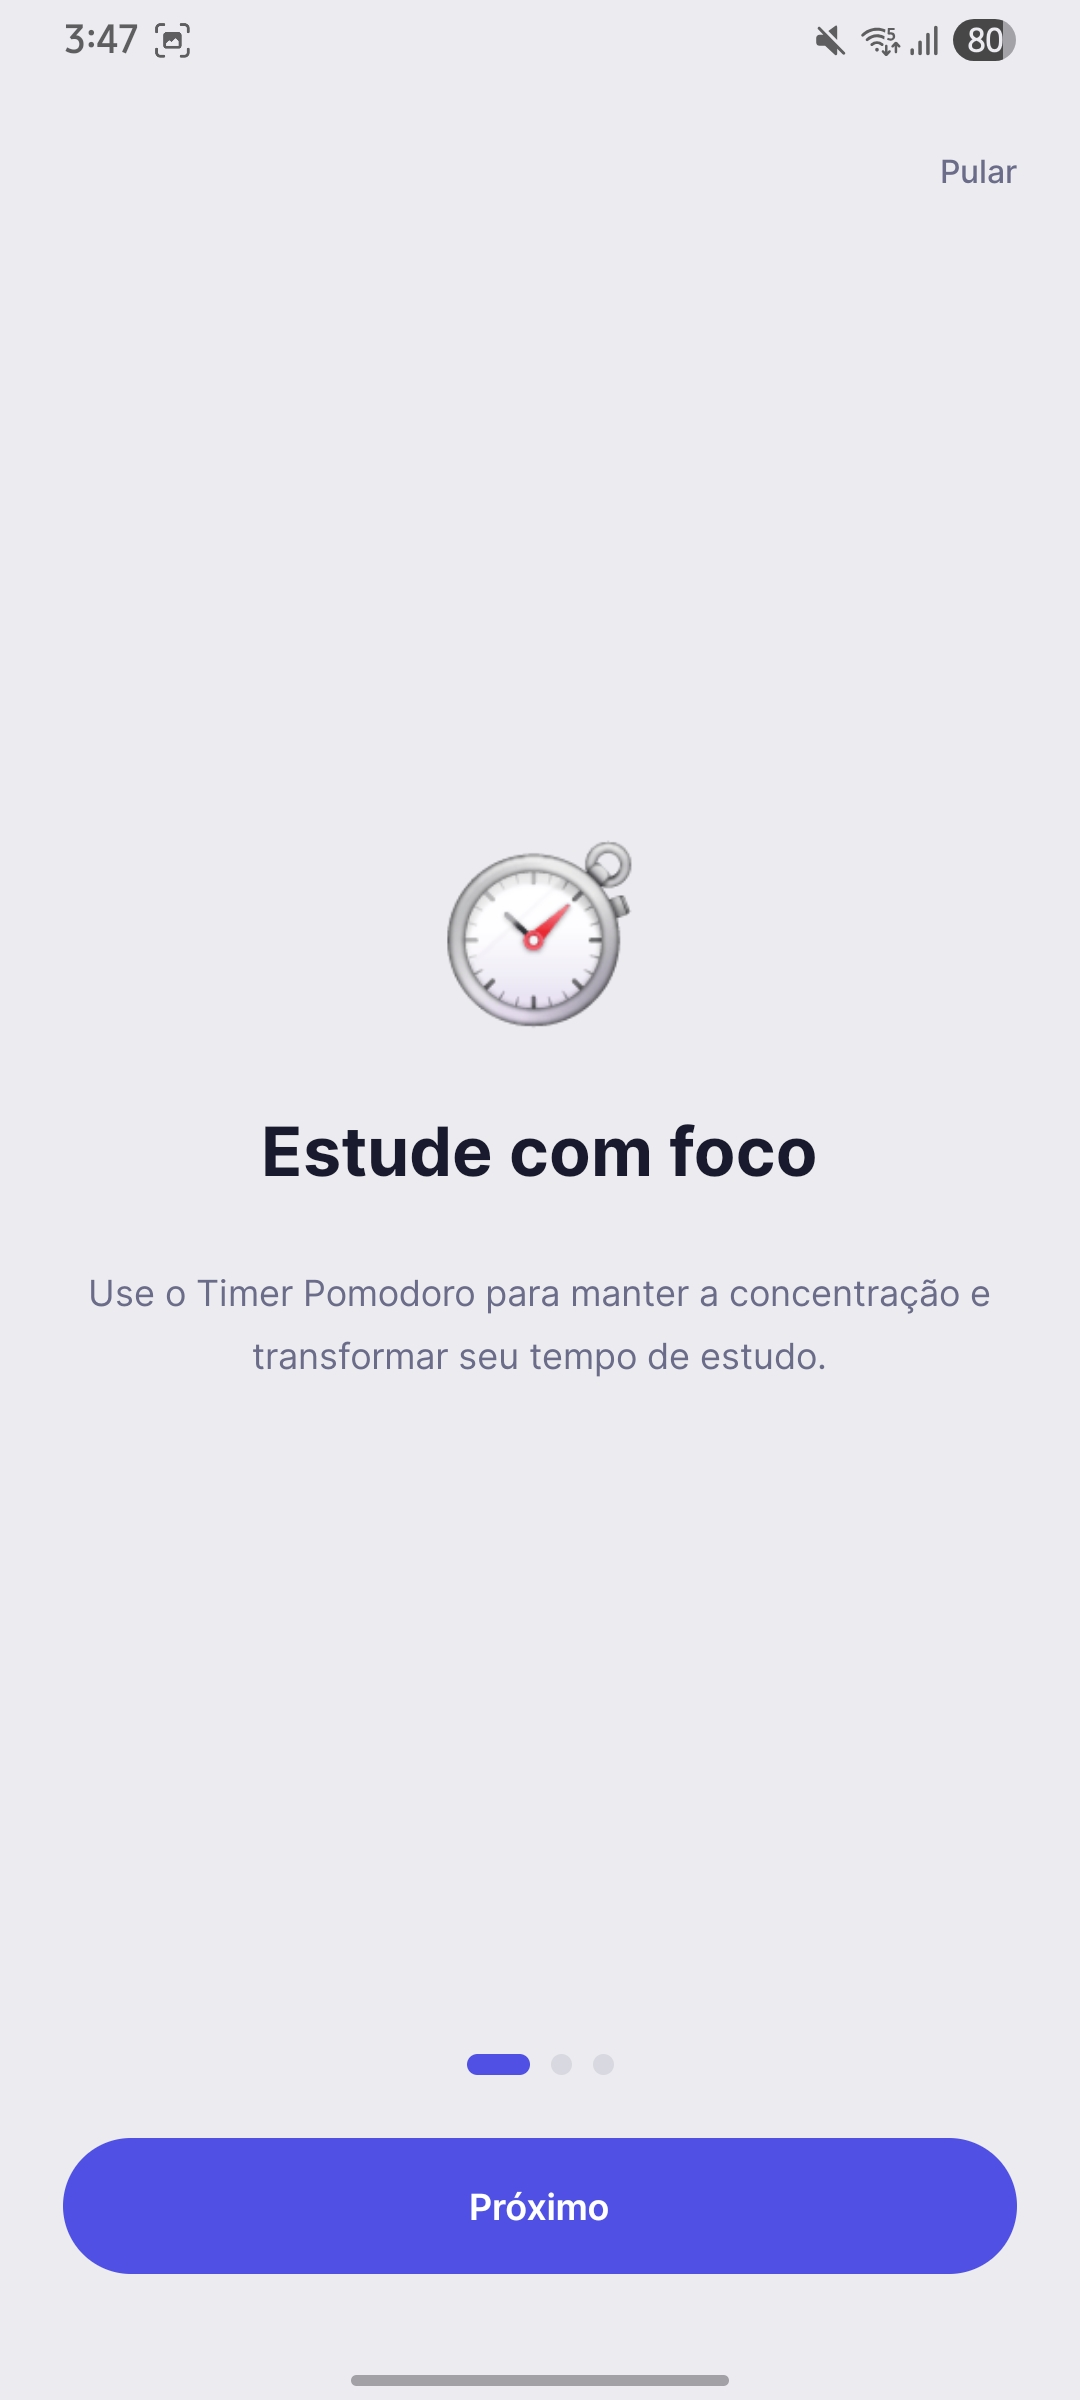
\includegraphics[height=0.7\textheight]{Imagens/PrototipoFigma/01_onboarding_metodo.jpg}
    \par
    Fonte: autoria própria.
    \par
    \label{p2}
\end{figure}

\begin{figure}[H]
    \centering
    \caption{Tela de Onboarding 2.}
    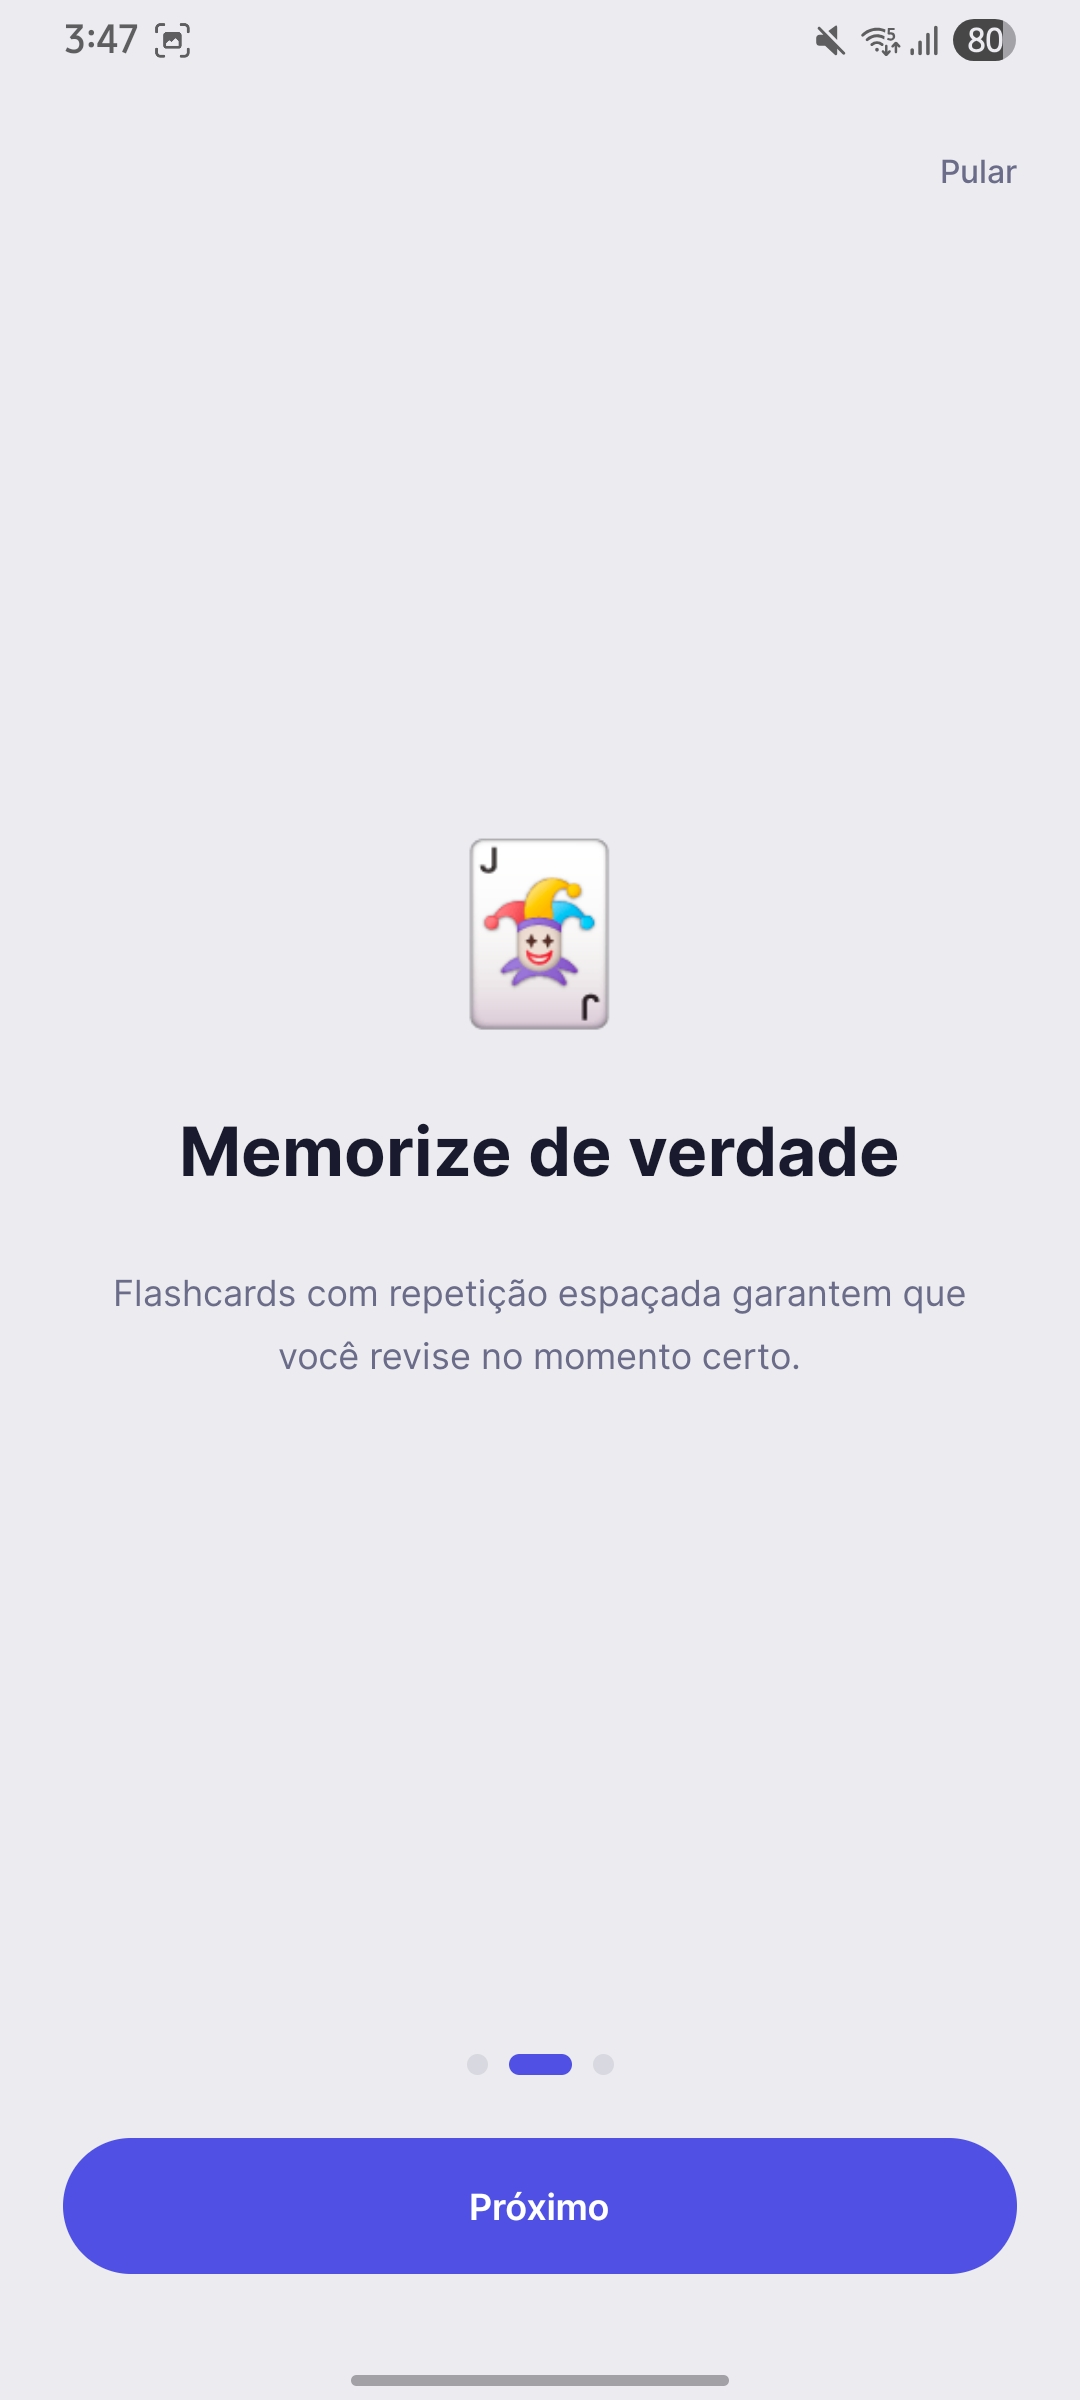
\includegraphics[height=0.7\textheight]{Imagens/PrototipoFigma/02_onboarding_srs.jpg}
    \par
    Fonte: autoria própria.
    \par
    \label{p3}
\end{figure}

\begin{figure}[H]
    \centering
    \caption{Tela de Onboarding 3.}
    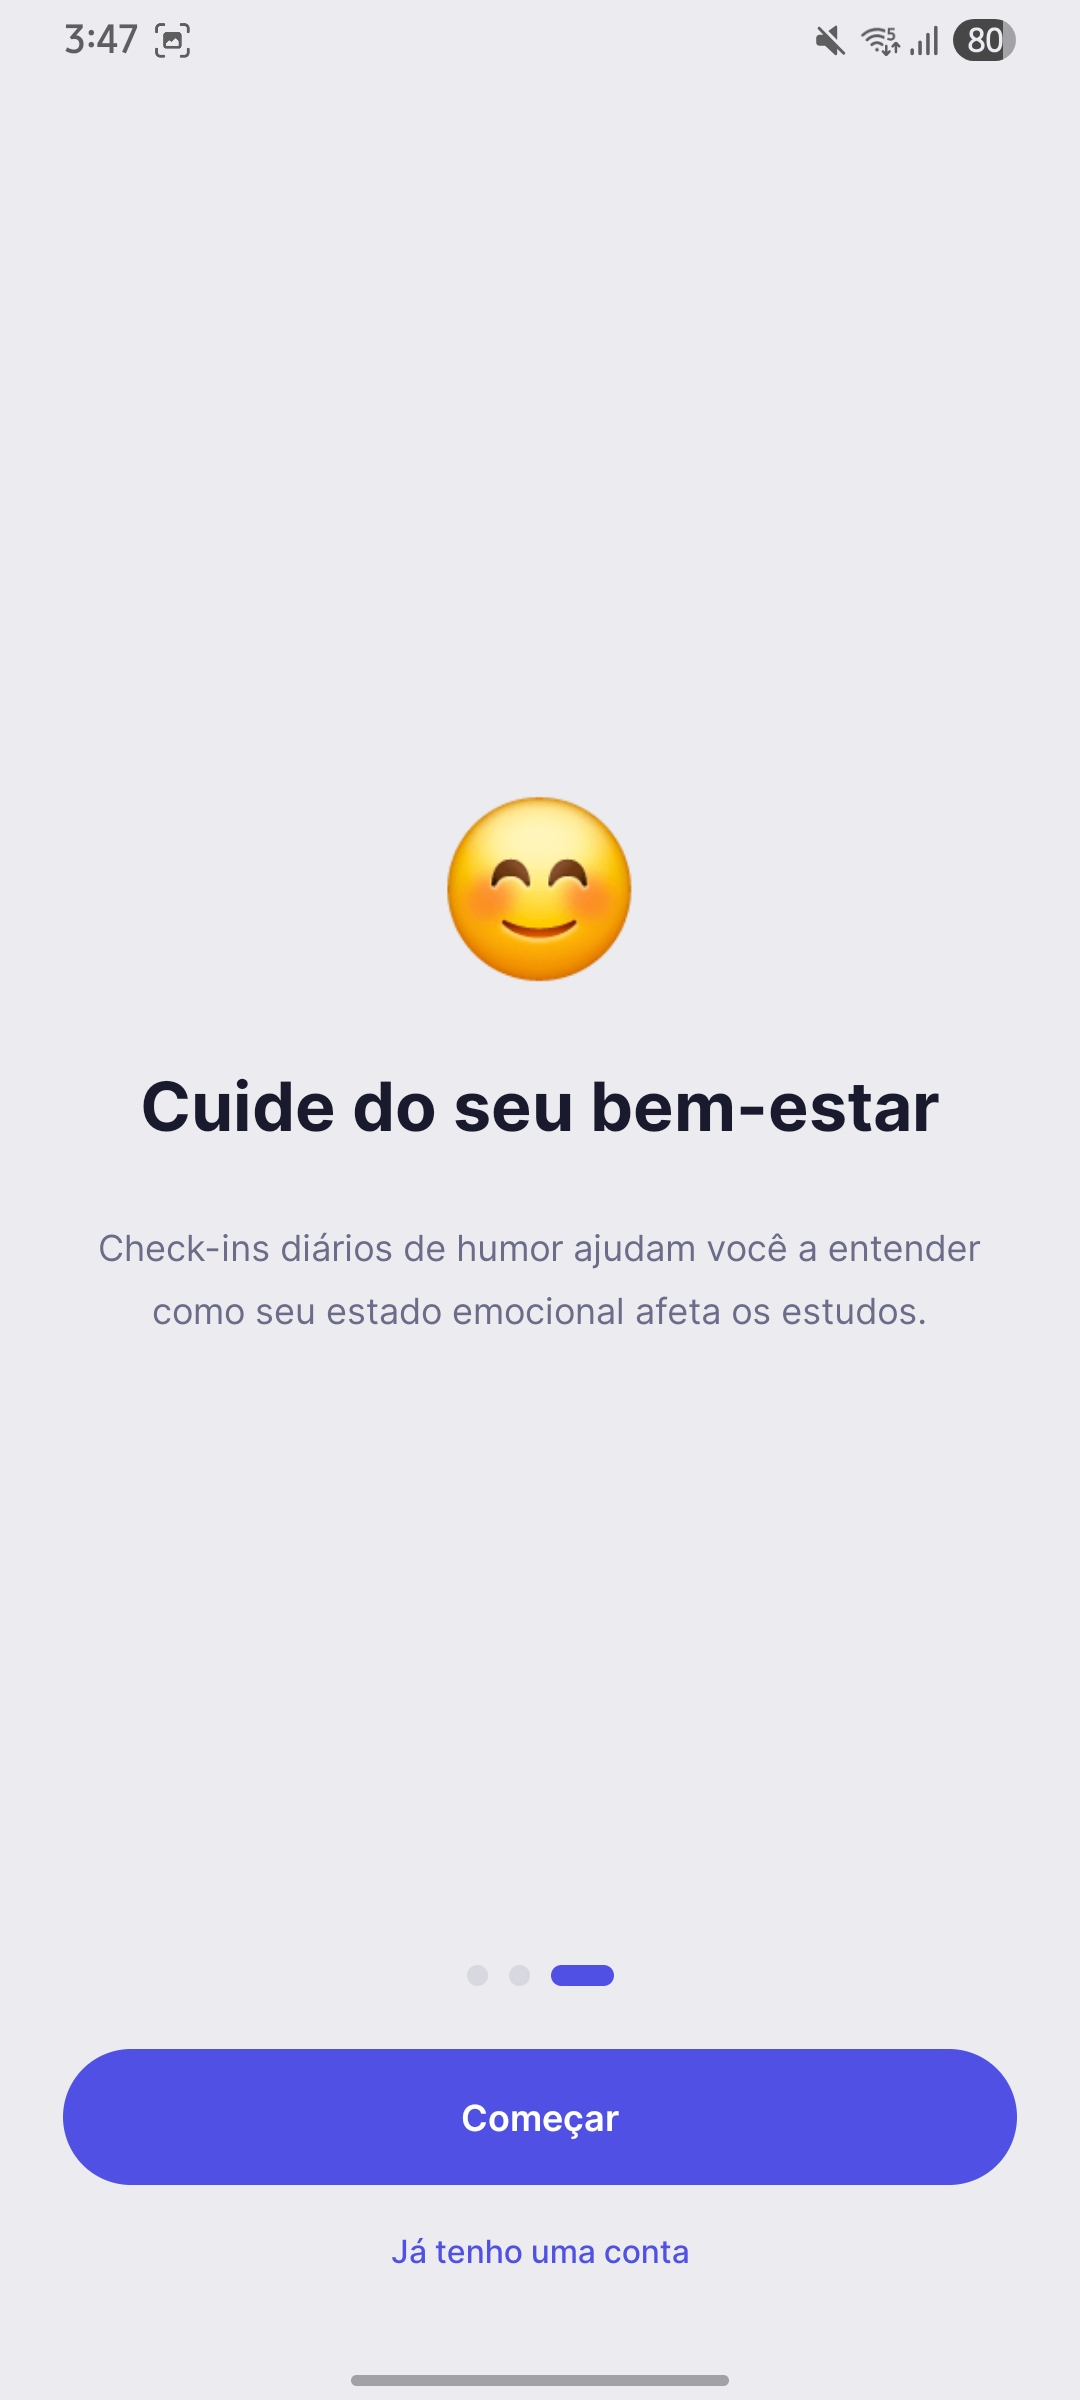
\includegraphics[height=0.7\textheight]{Imagens/PrototipoFigma/03_onboarding_bemestar.jpg}
    \par
    Fonte: autoria própria.
    \par
    \label{p4}
\end{figure}

\begin{figure}[H]
    \centering
    \caption{Tela de Criar Conta.}
    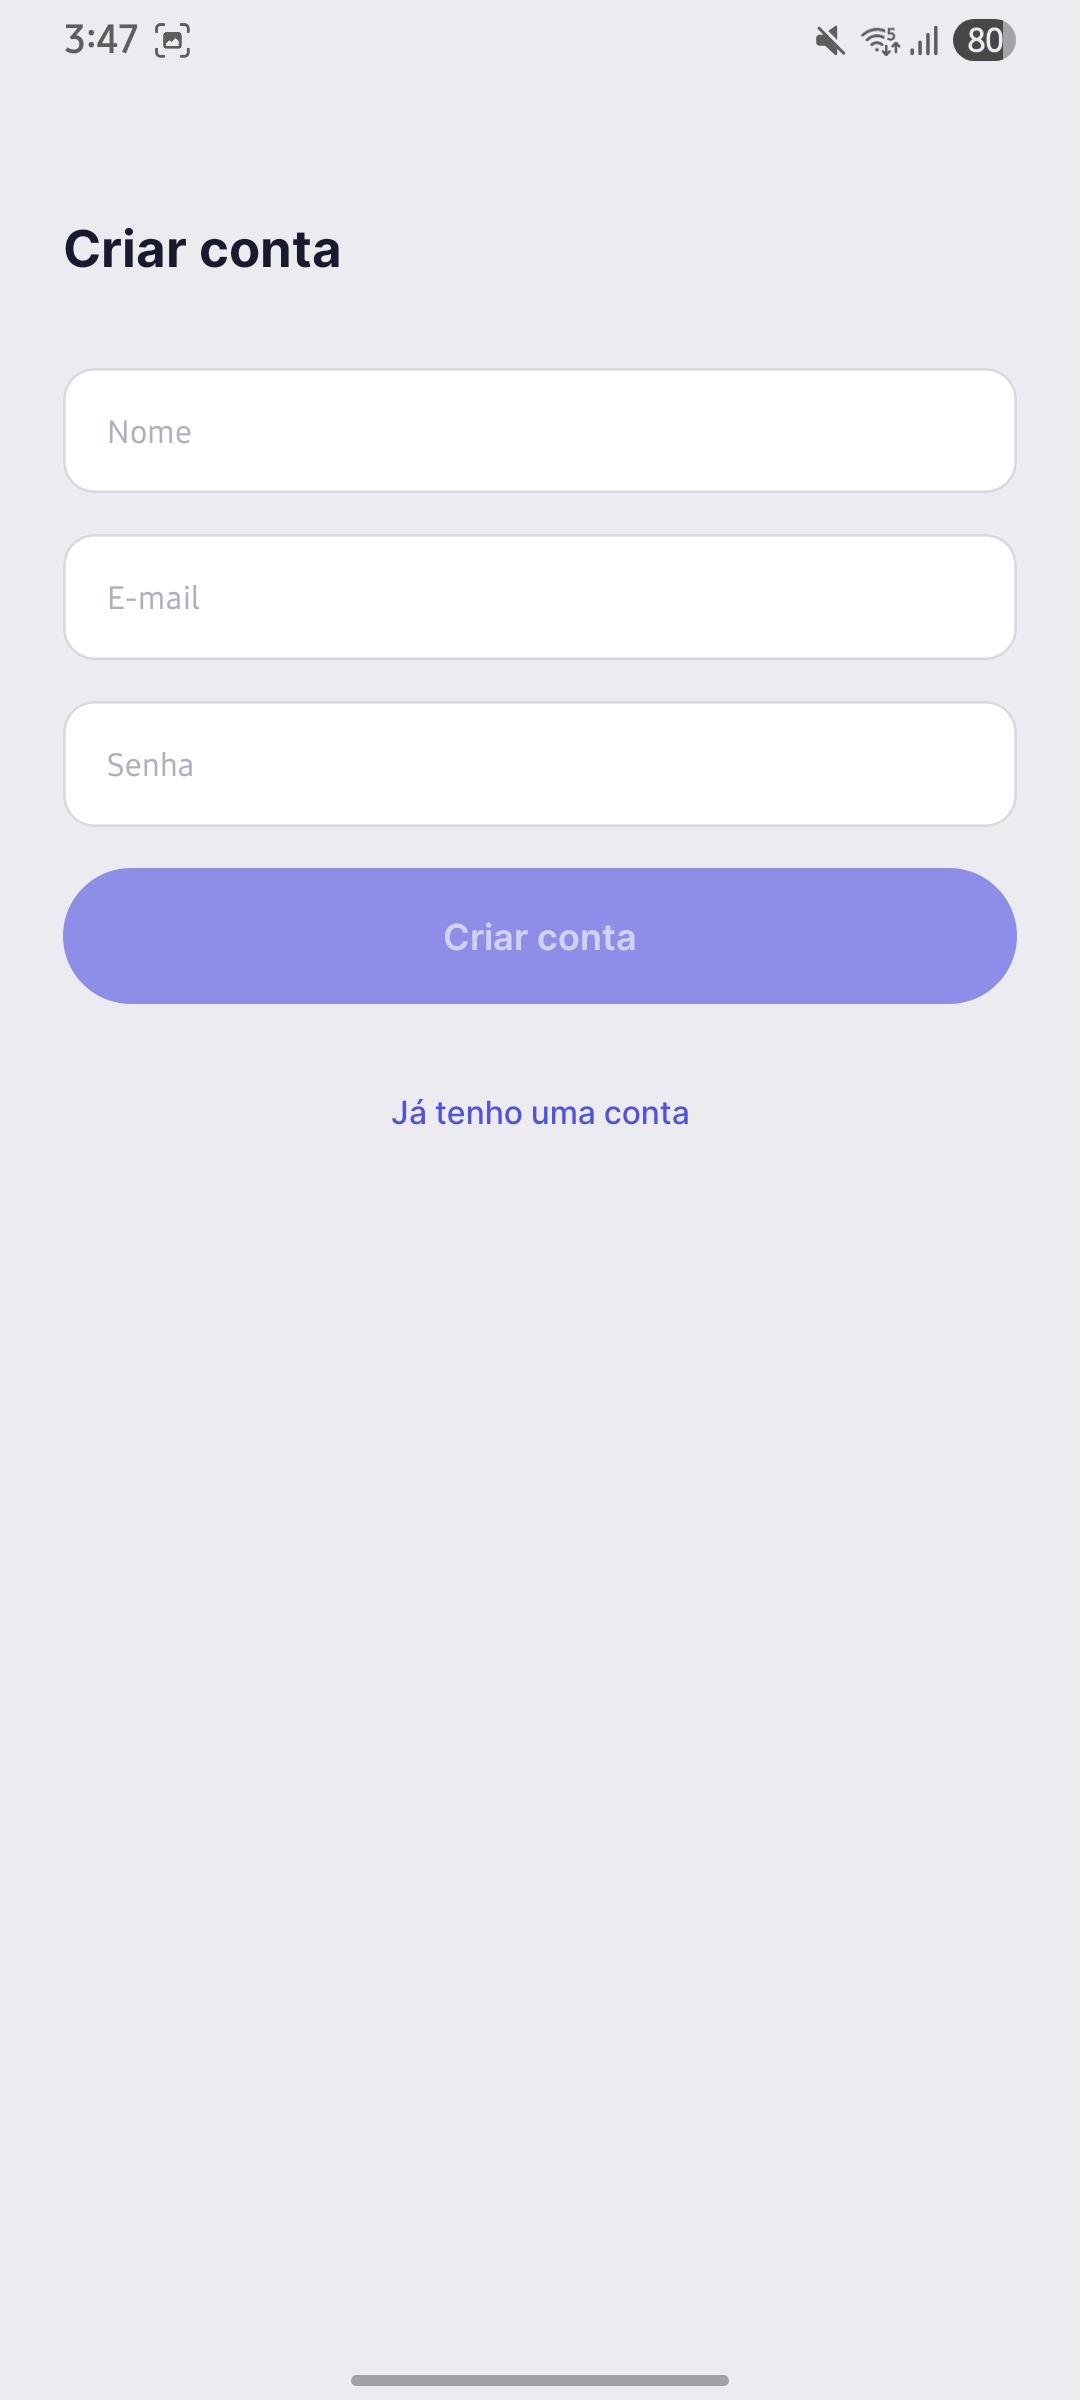
\includegraphics[height=0.7\textheight]{Imagens/PrototipoFigma/04_signup.jpg}
    \par
    Fonte: autoria própria.
    \par
    \label{p5}
\end{figure}

\begin{figure}[H]
    \centering
    \caption{Tela de Login.}
    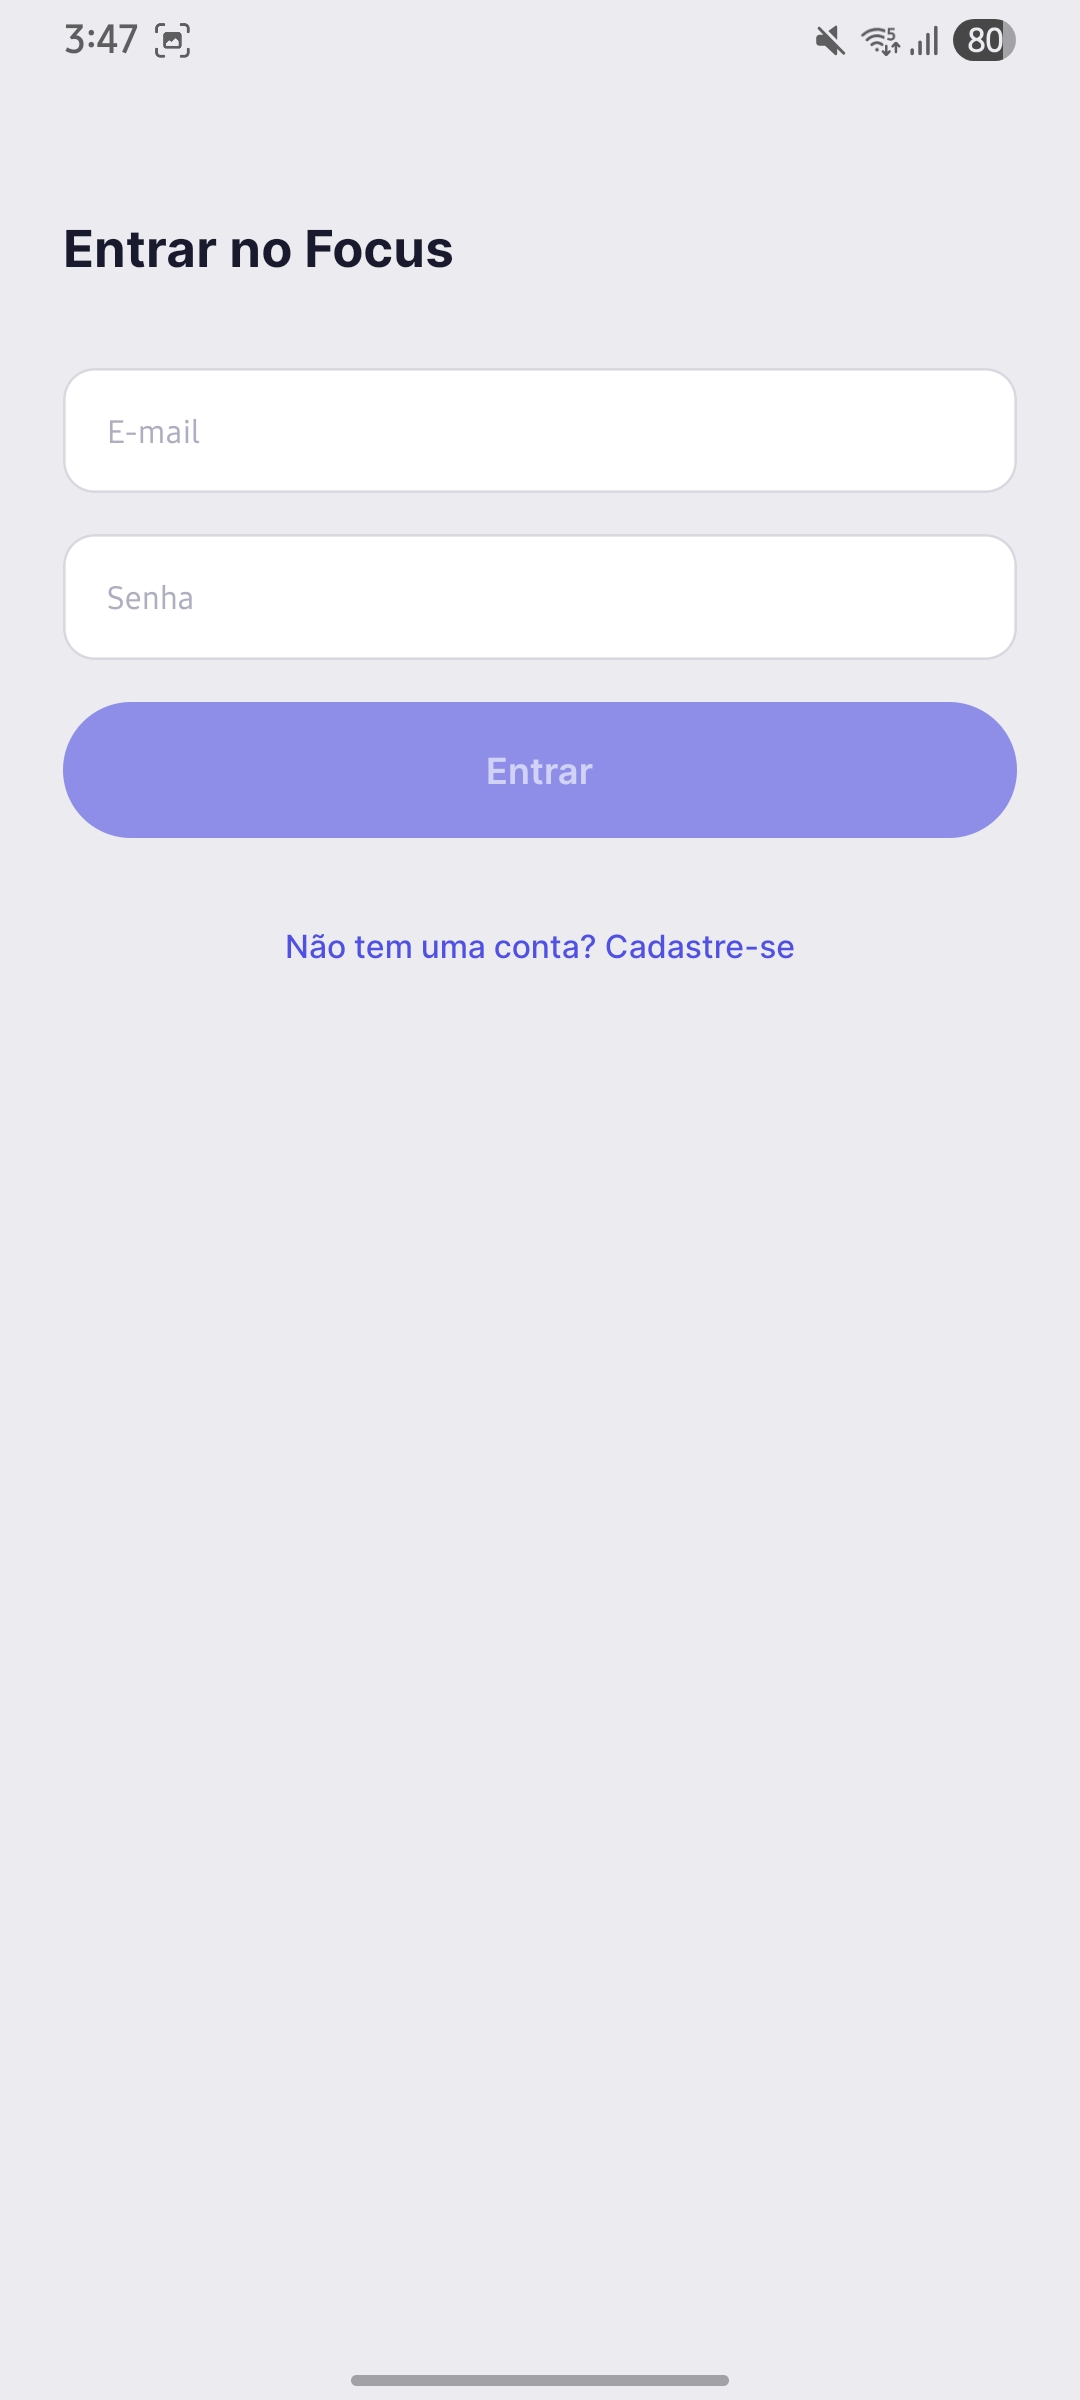
\includegraphics[height=0.7\textheight]{Imagens/PrototipoFigma/05_login.jpg}
    \par
    Fonte: autoria própria.
    \par
    \label{p6}
\end{figure}

\begin{figure}[H]
    \centering
    \caption{Tela de Home.}
    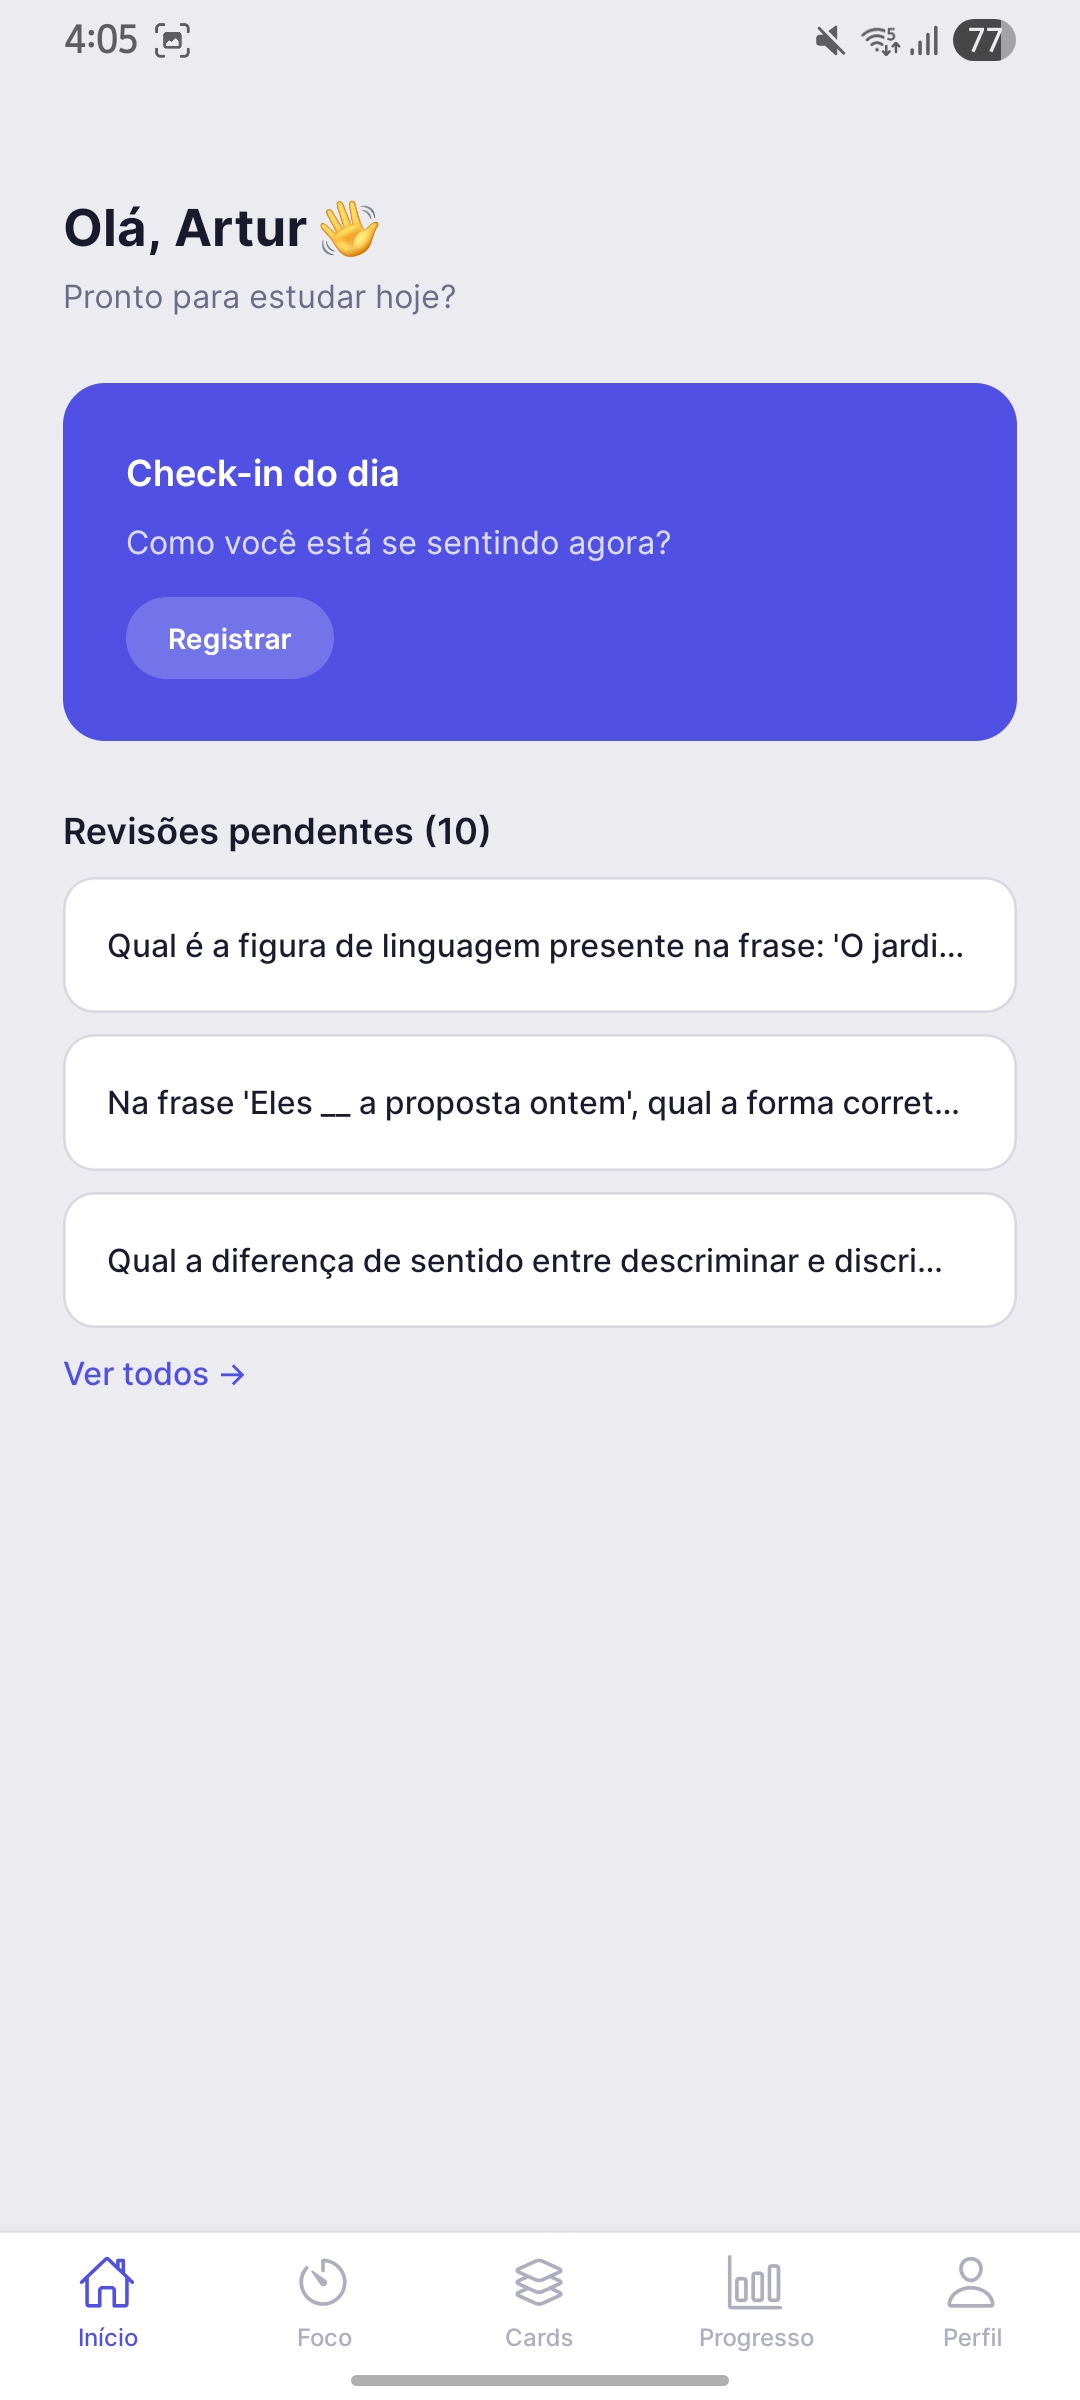
\includegraphics[height=0.7\textheight]{Imagens/PrototipoFigma/06_home.jpg}
    \par
    Fonte: autoria própria.
    \par
    \label{p7}
\end{figure}

\begin{figure}[H]
    \centering
    \caption{Tela do Timer.}
    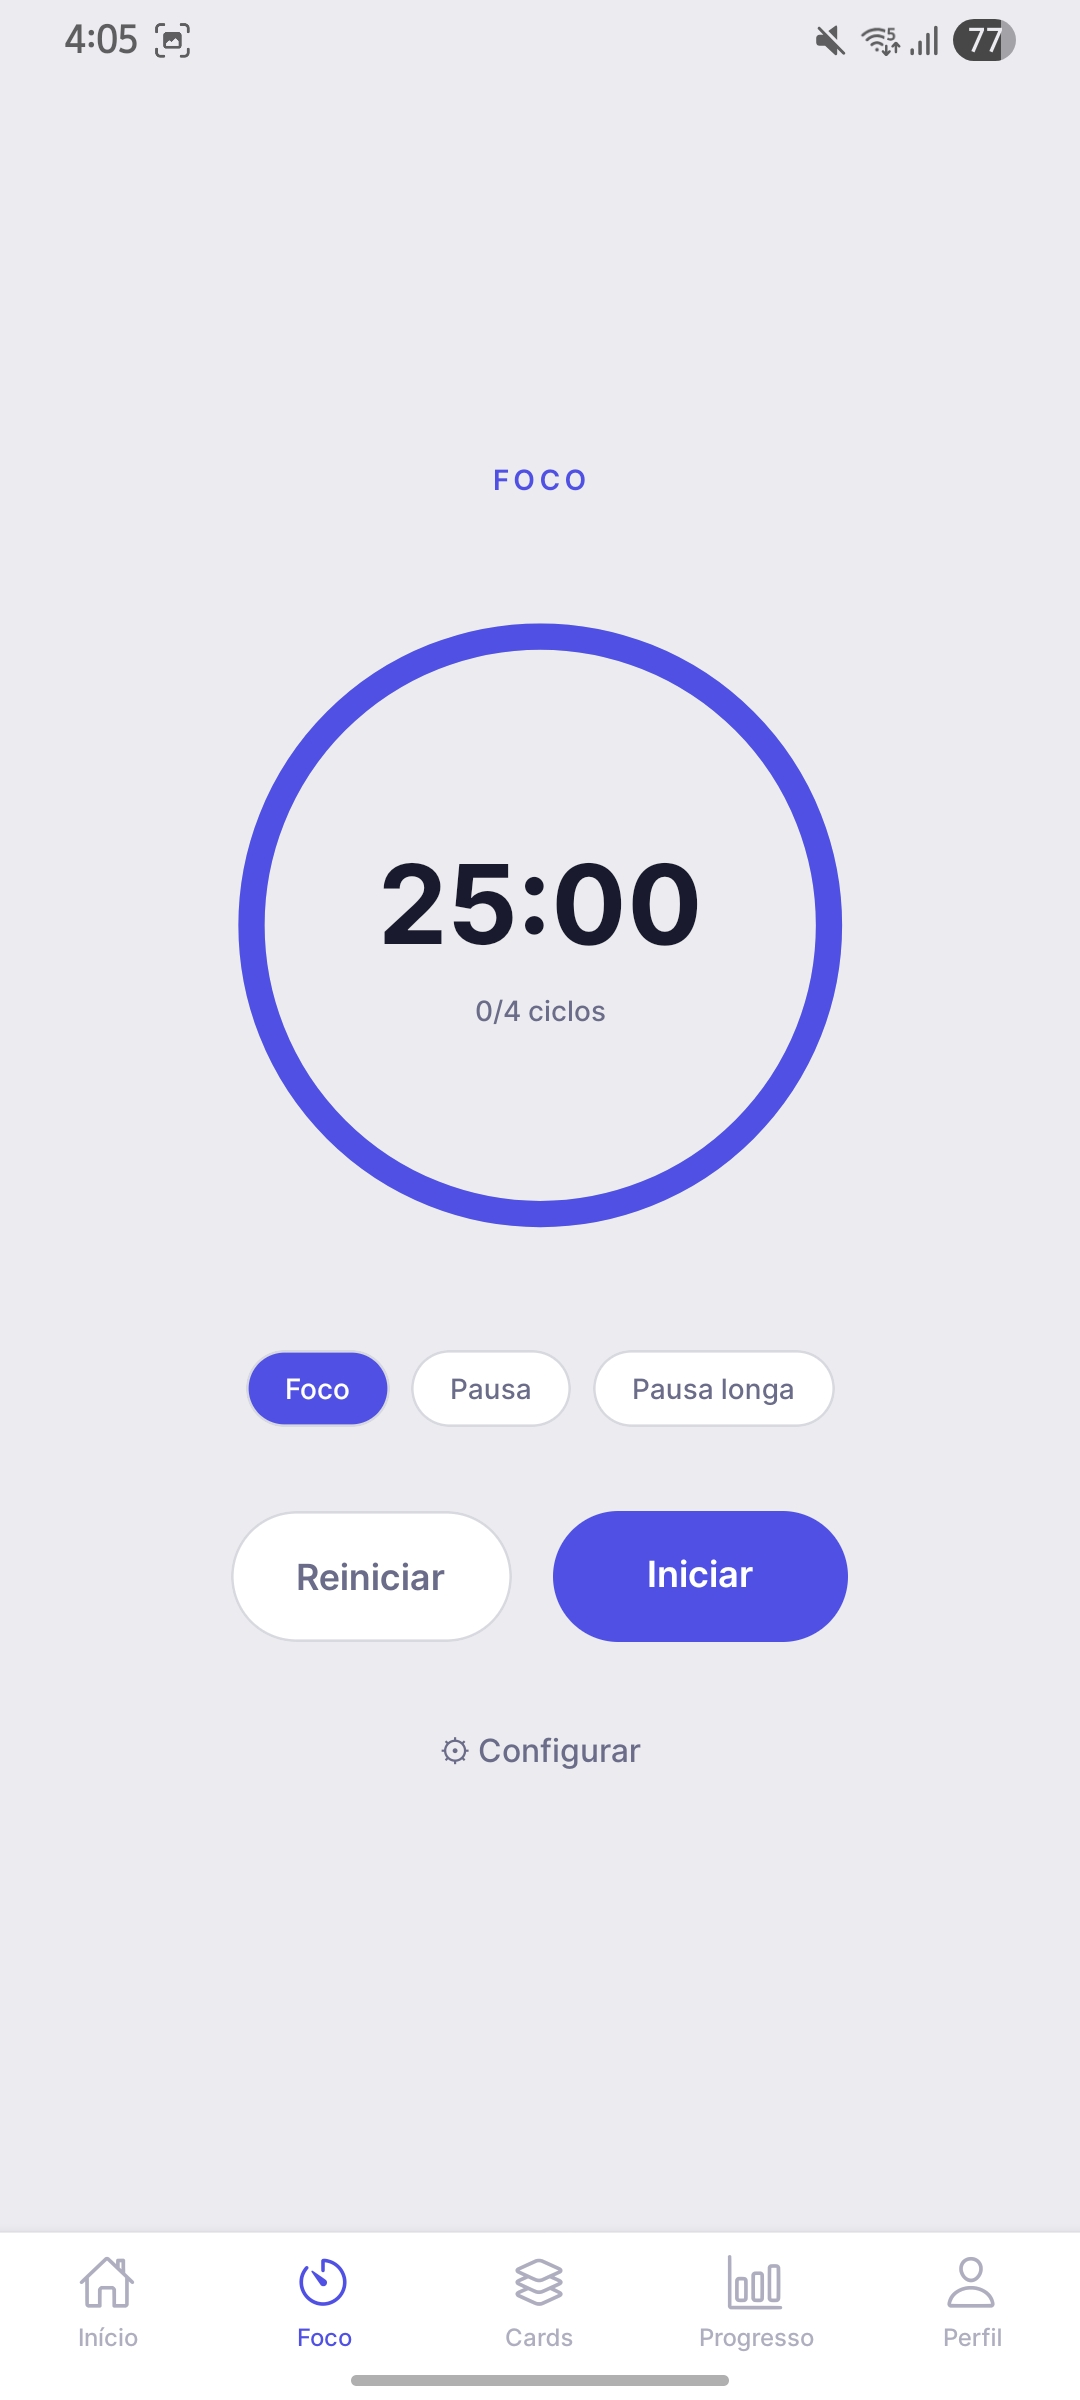
\includegraphics[height=0.7\textheight]{Imagens/PrototipoFigma/07_timer.jpg}
    \par
    Fonte: autoria própria.
    \par
    \label{p8}
\end{figure}

\begin{figure}[H]
    \centering
    \caption{Tela de Configurações do Timer.}
    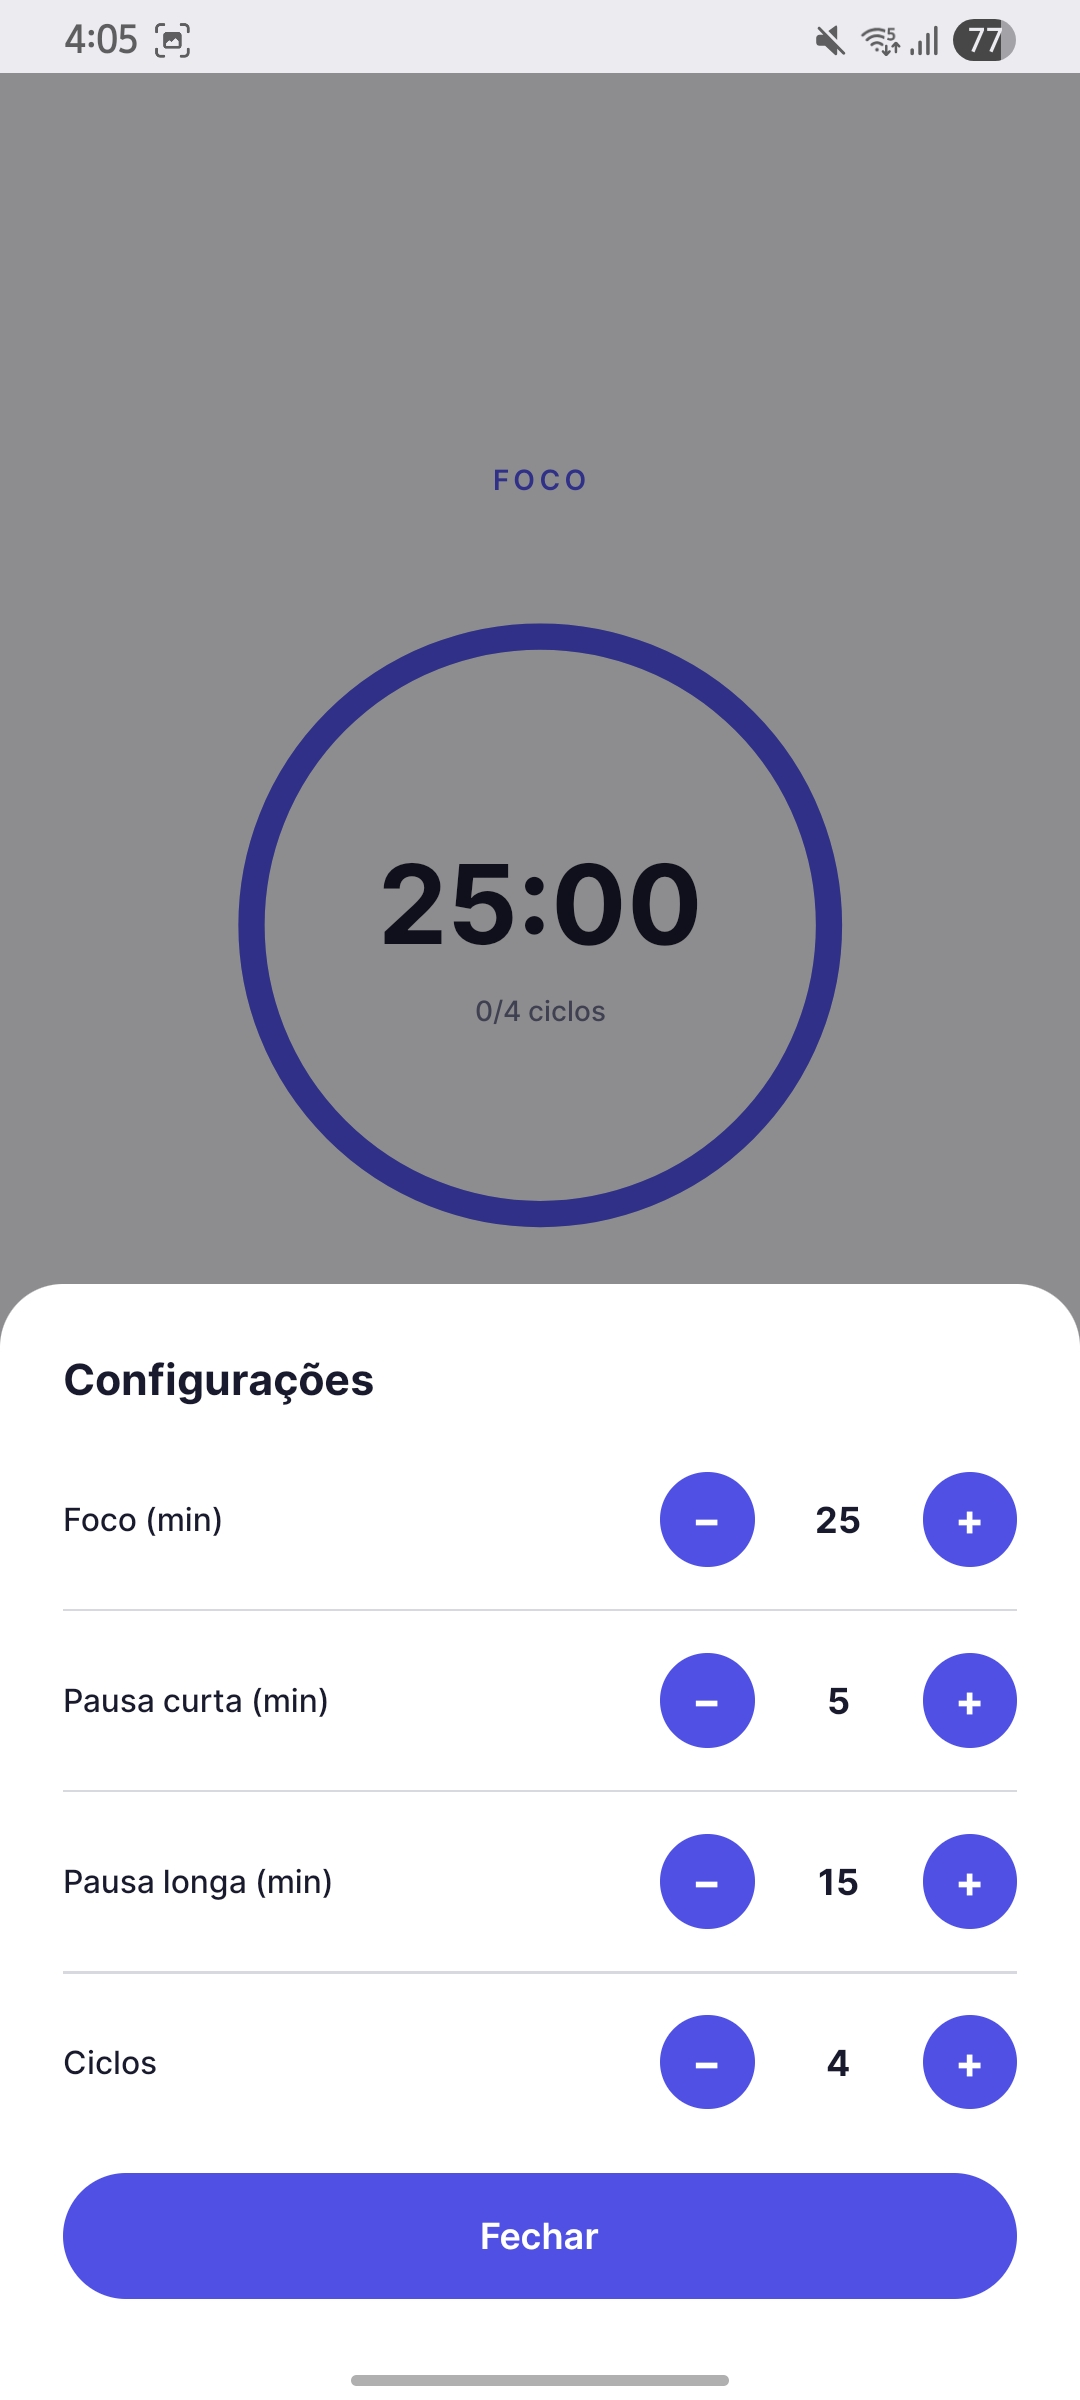
\includegraphics[height=0.7\textheight]{Imagens/PrototipoFigma/08_timer_settings.jpg}
    \par
    Fonte: autoria própria.
    \par
    \label{p9}
\end{figure}

\begin{figure}[H]
    \centering
    \caption{Tela de Novo Flashcard.}
    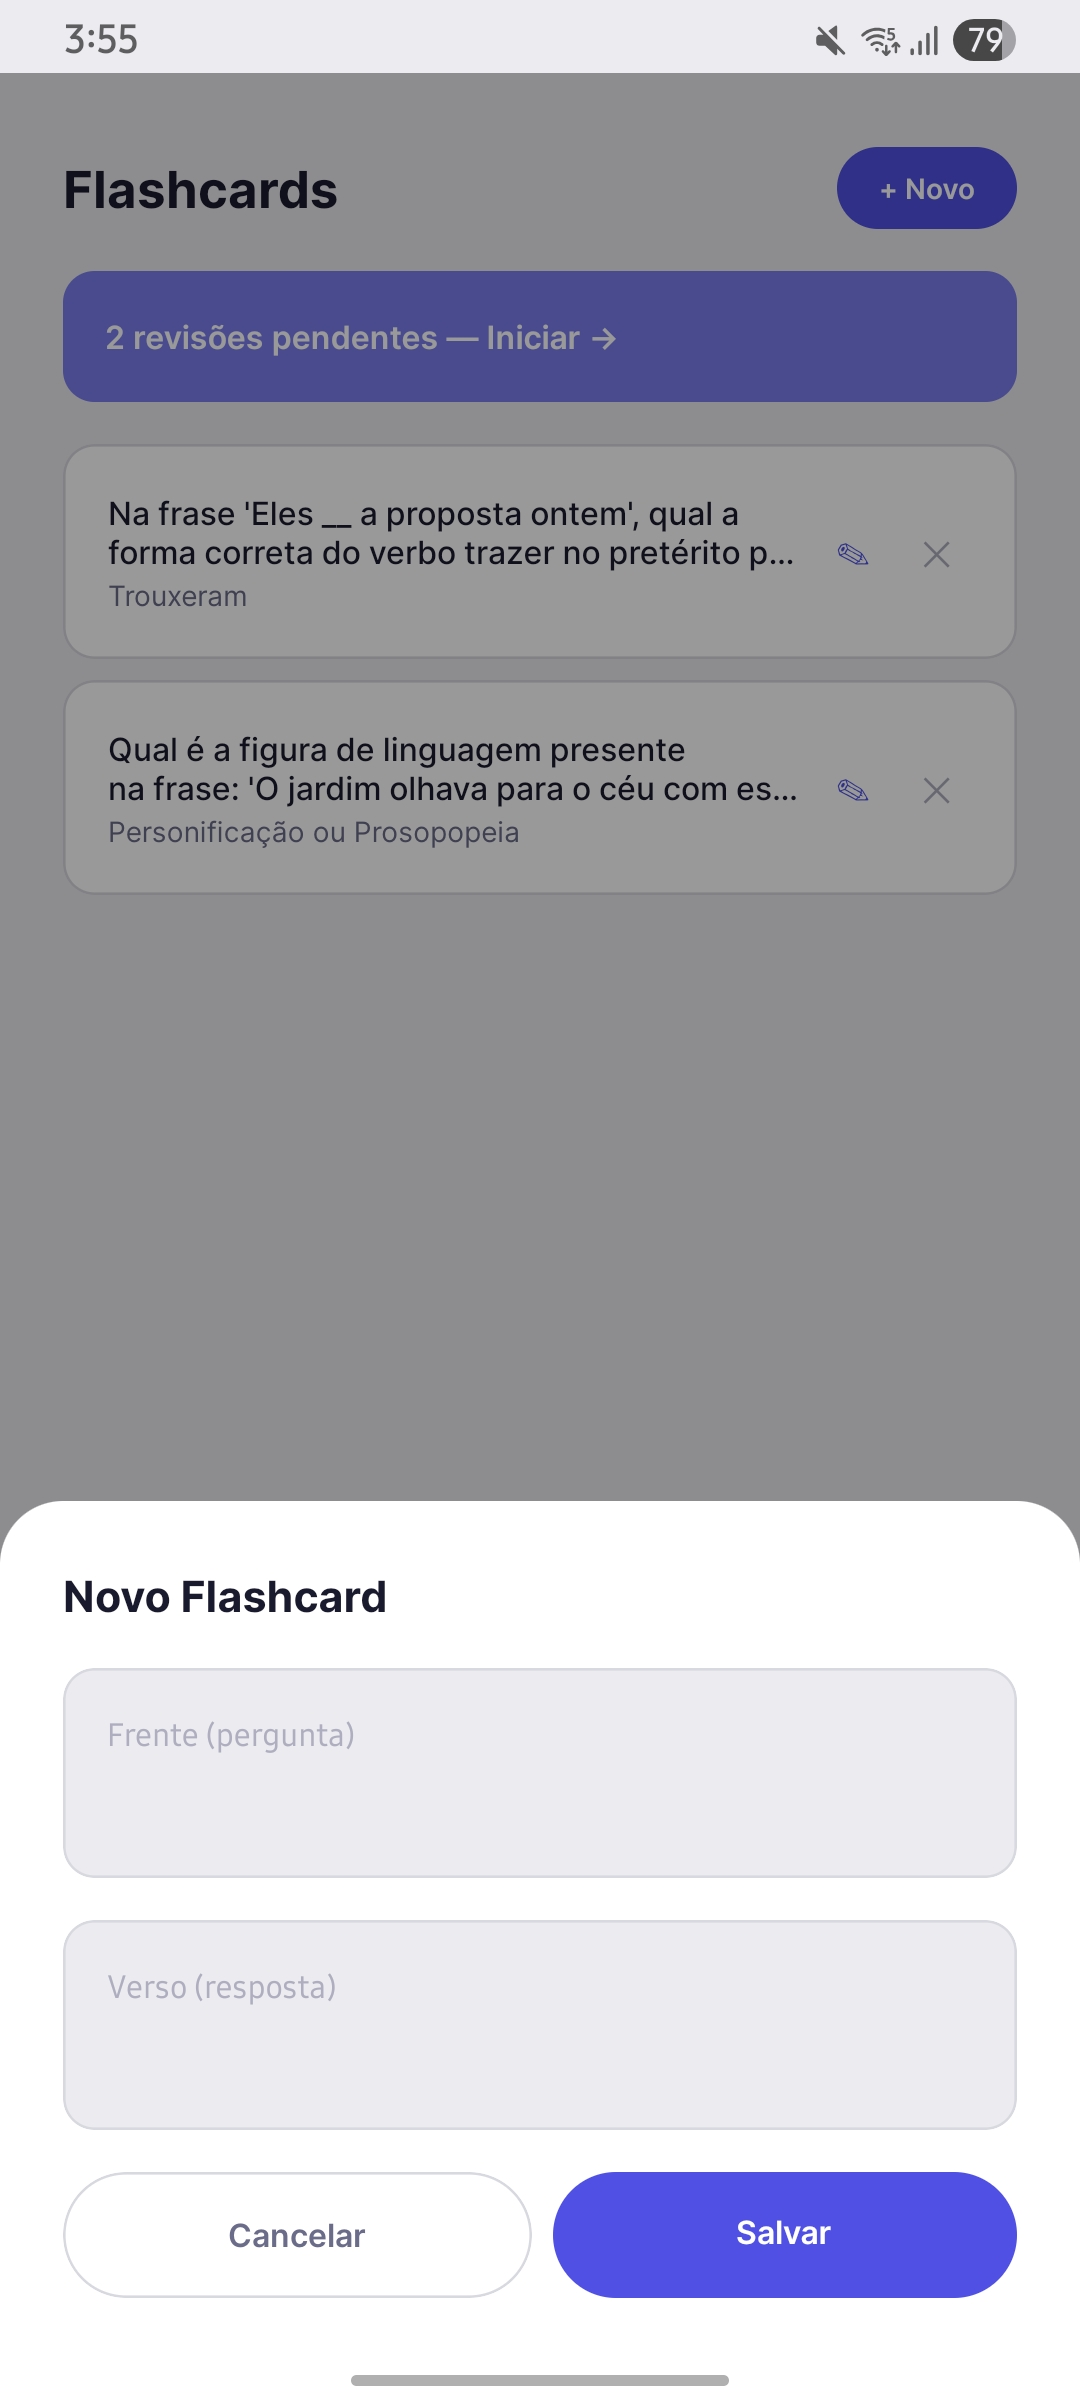
\includegraphics[height=0.7\textheight]{Imagens/PrototipoFigma/09_new_flashcard.jpg}
    \par
    Fonte: autoria própria.
    \par
    \label{p10}
\end{figure}

\begin{figure}[H]
    \centering
    \caption{Tela de Flashcards.}
    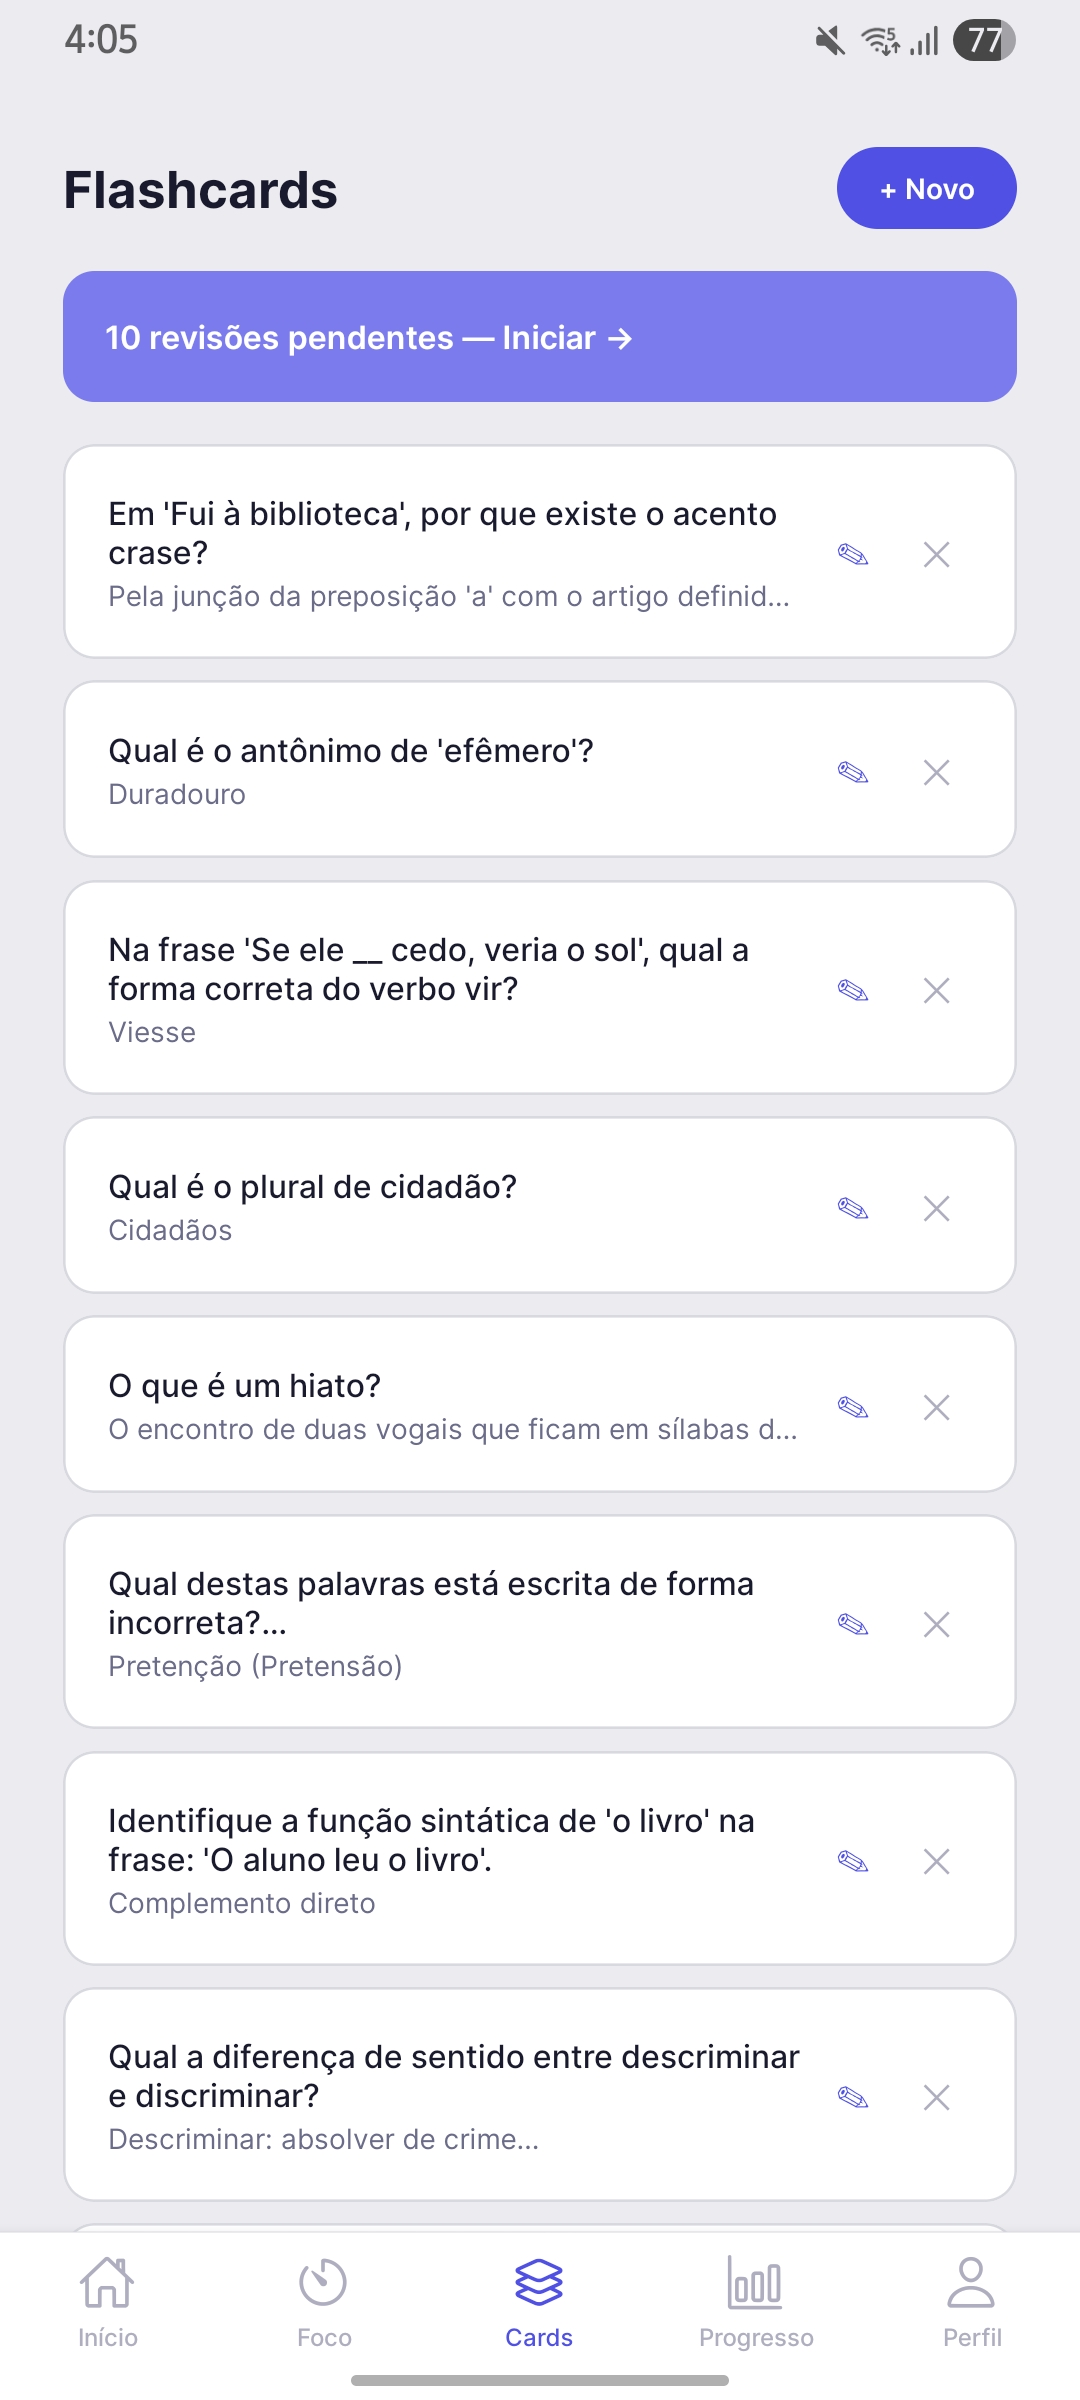
\includegraphics[height=0.7\textheight]{Imagens/PrototipoFigma/10_flashcards.jpg}
    \par
    Fonte: autoria própria.
    \par
    \label{p11}
\end{figure}

\begin{figure}[H]
    \centering
    \caption{Tela de Exclusão de Flashcard.}
    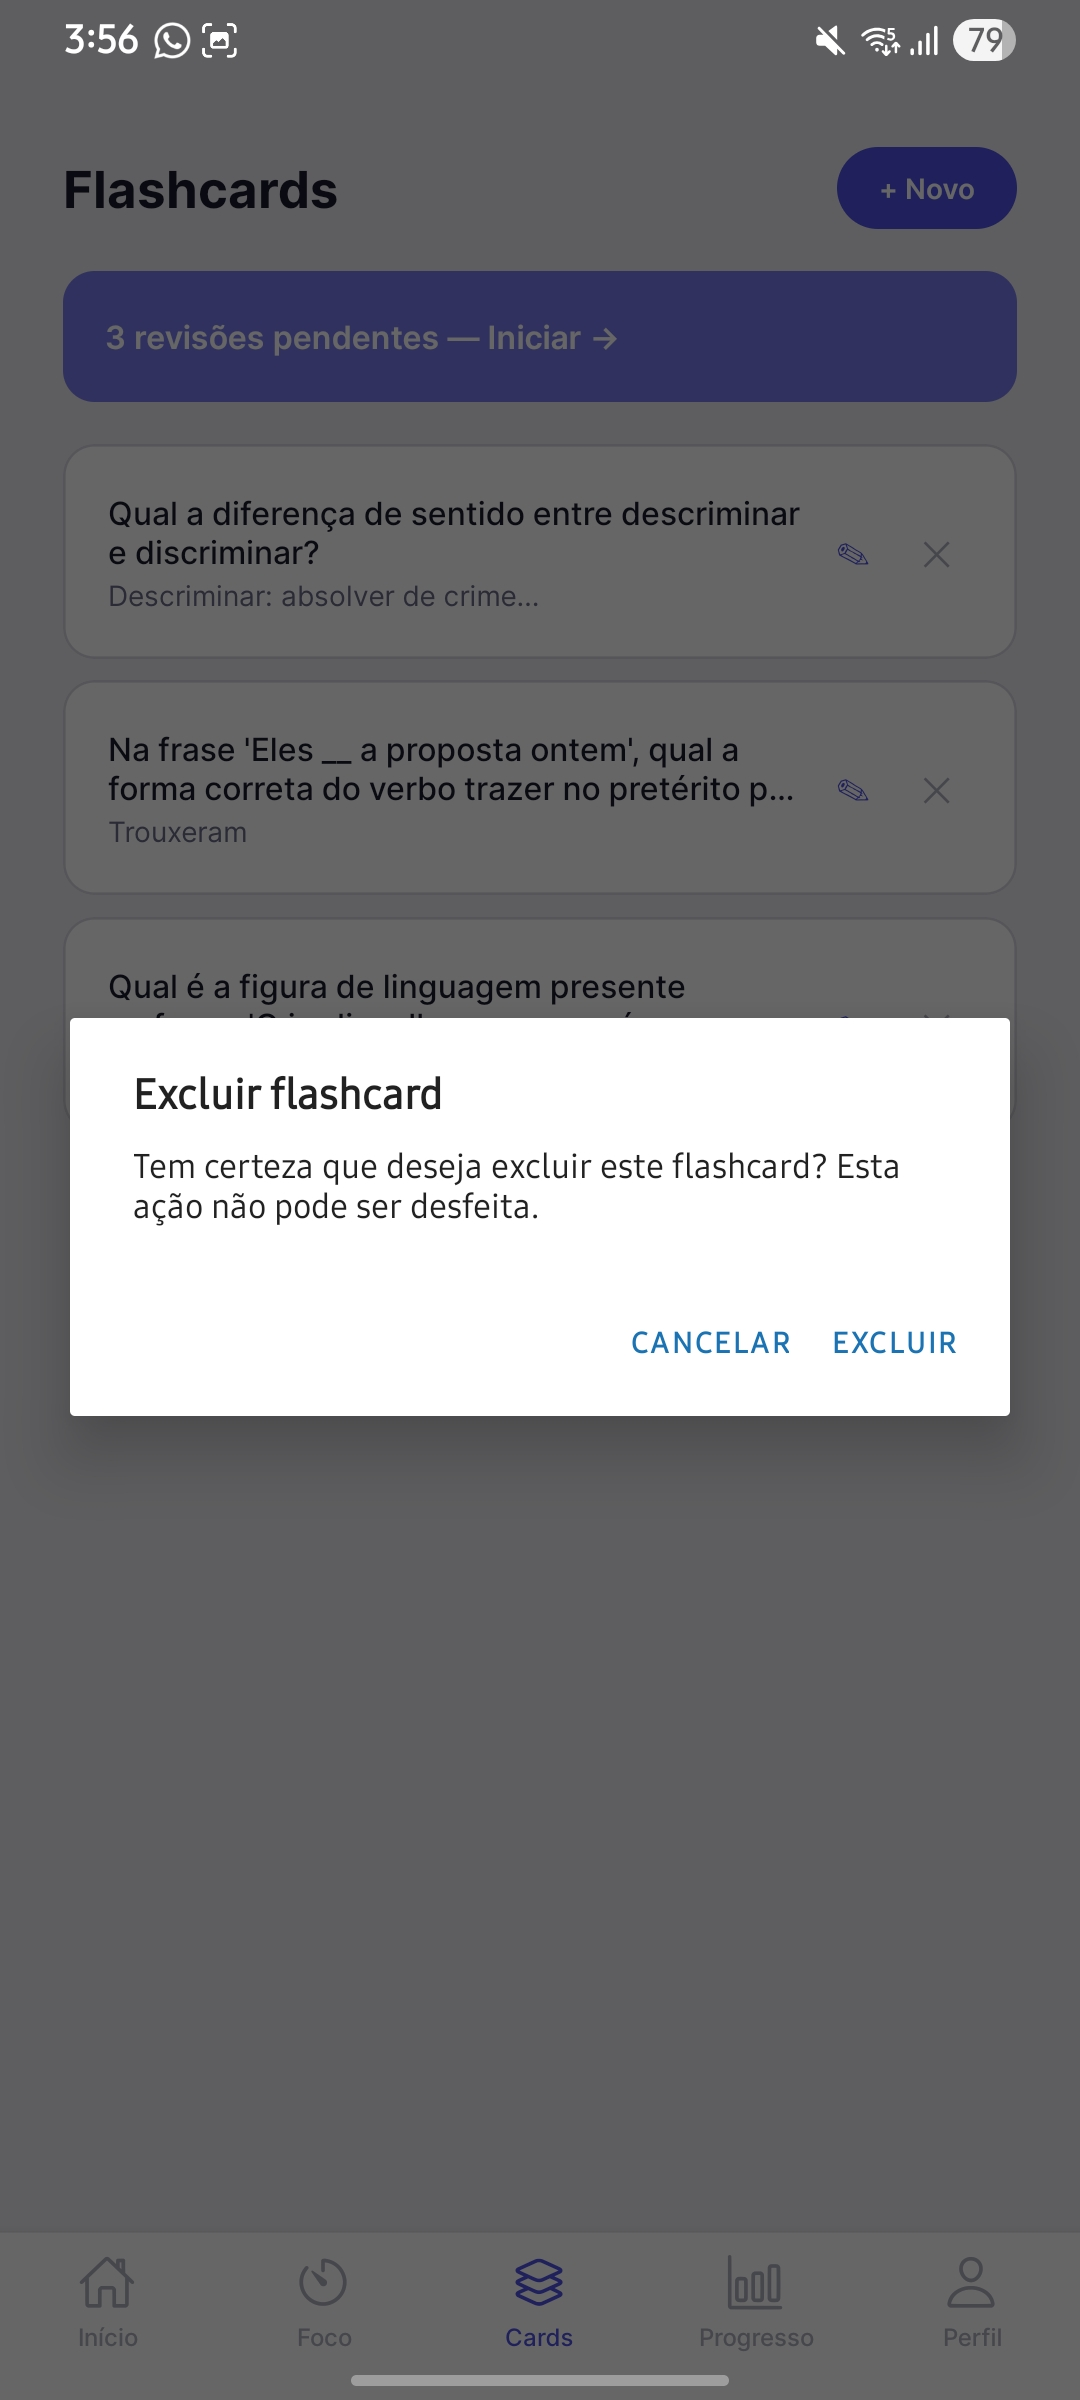
\includegraphics[height=0.7\textheight]{Imagens/PrototipoFigma/11_flashcard_delete.jpg}
    \par
    Fonte: autoria própria.
    \par
    \label{p12}
\end{figure}

\begin{figure}[H]
    \centering
    \caption{Tela de Revisão — Frente.}
    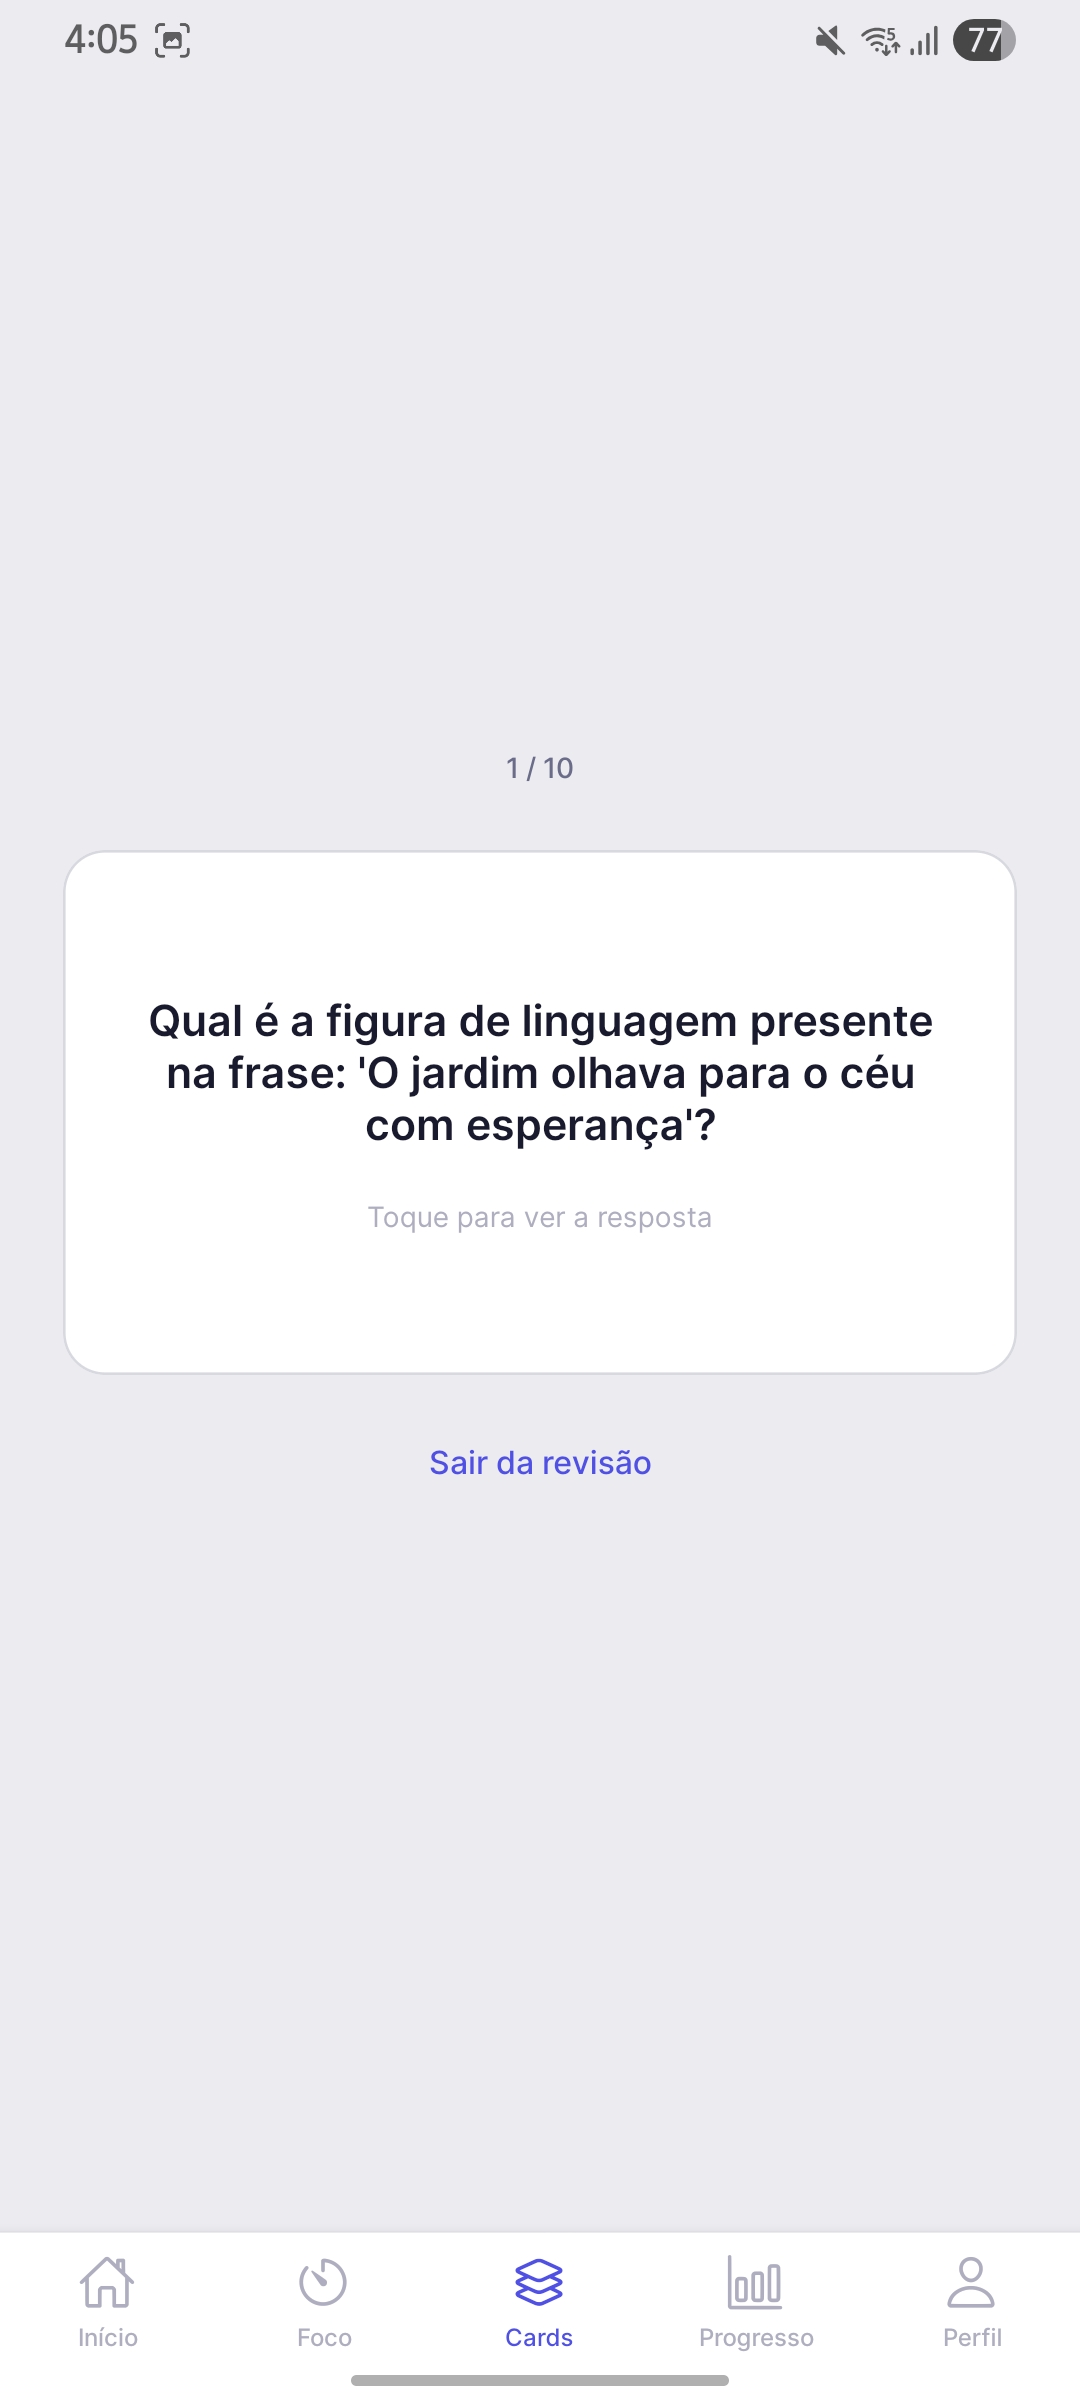
\includegraphics[height=0.7\textheight]{Imagens/PrototipoFigma/12_flashcard_front.jpg}
    \par
    Fonte: autoria própria.
    \par
    \label{p13}
\end{figure}

\begin{figure}[H]
    \centering
    \caption{Tela de Revisão — Verso.}
    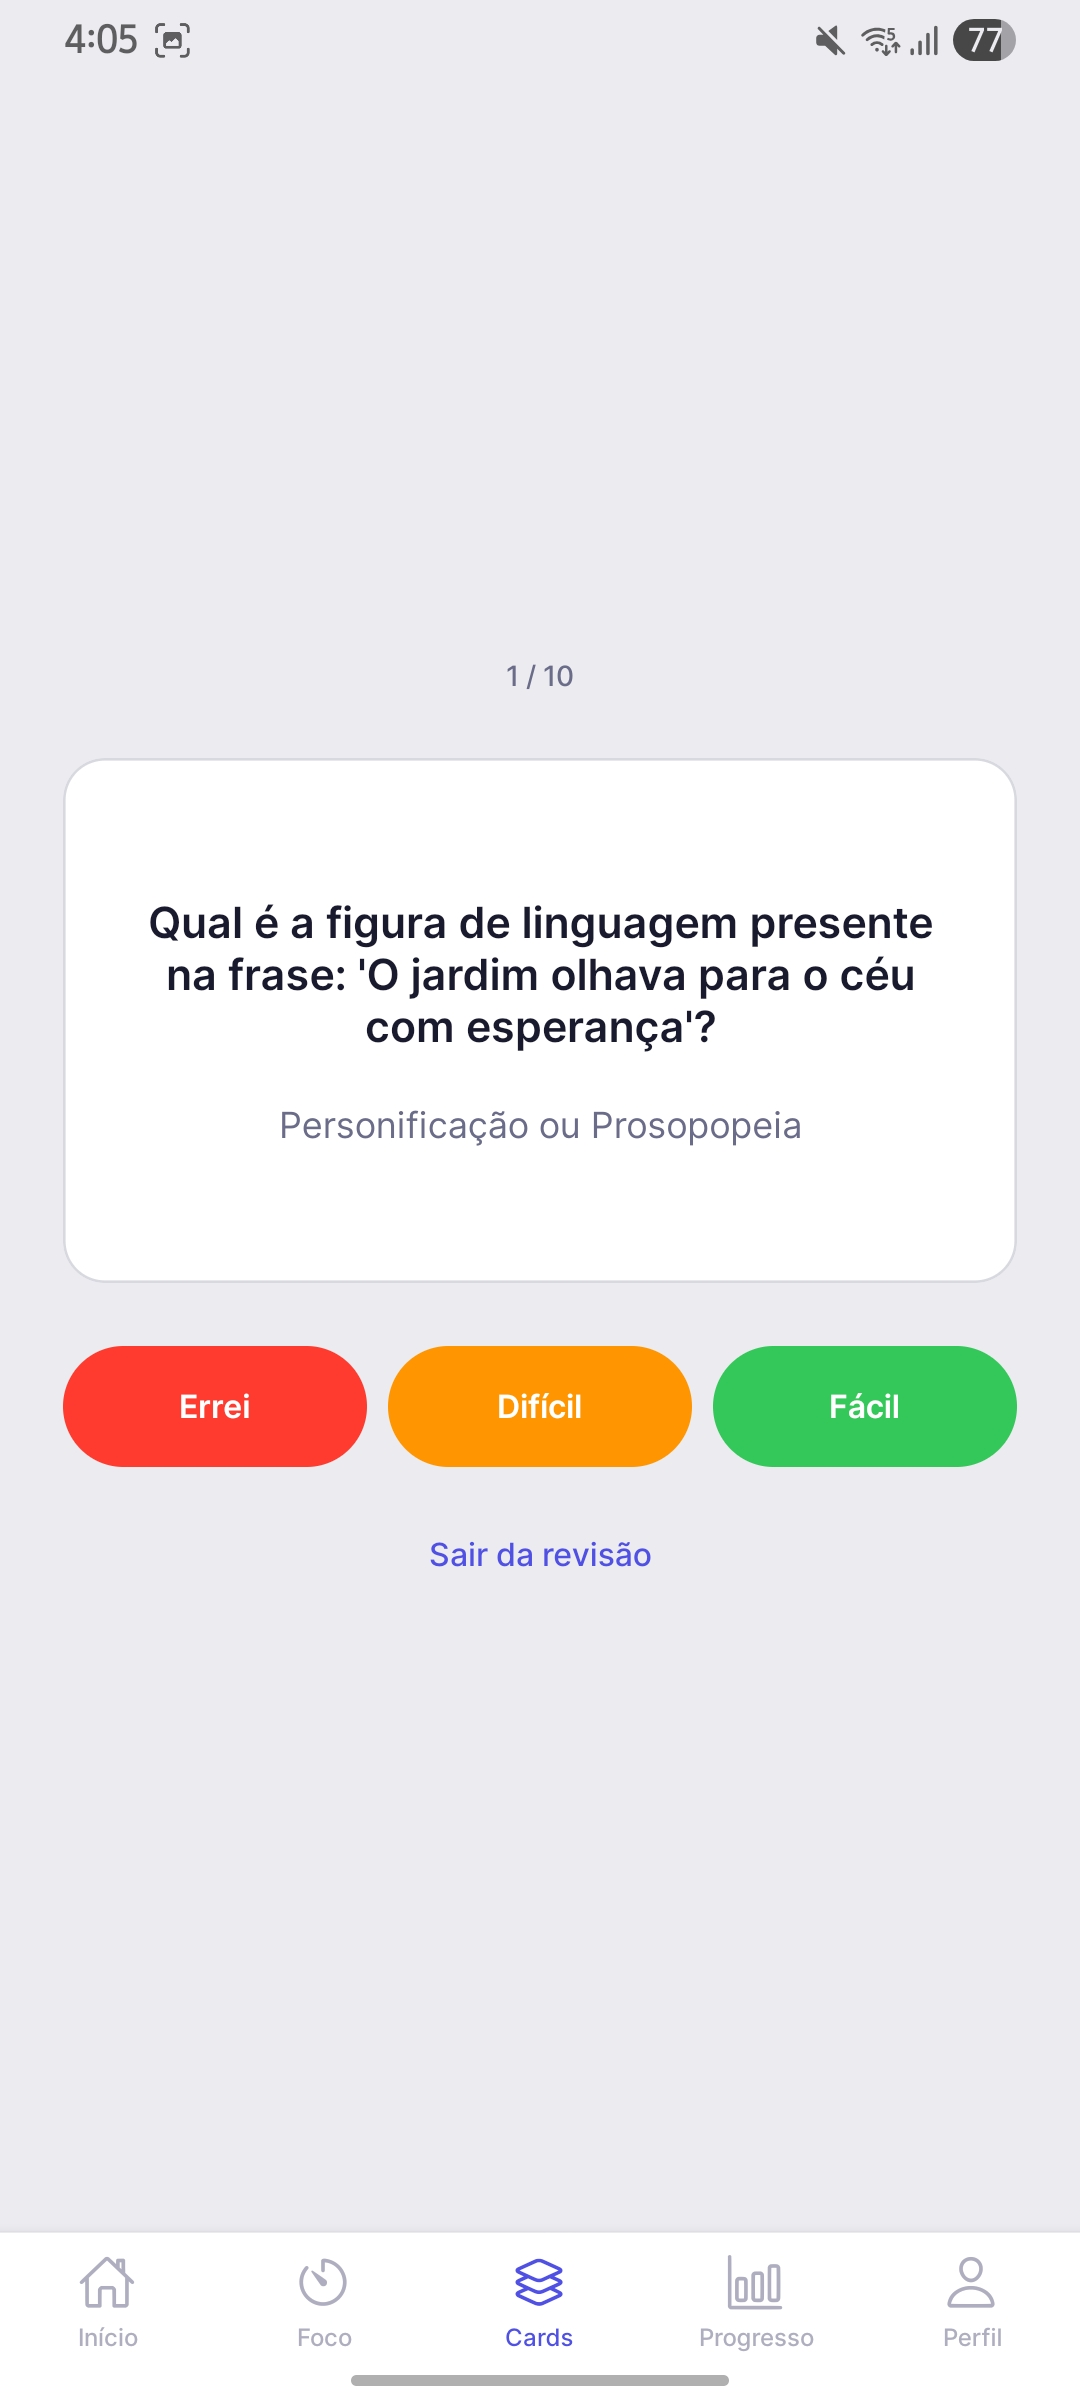
\includegraphics[height=0.7\textheight]{Imagens/PrototipoFigma/13_flashcard_back.jpg}
    \par
    Fonte: autoria própria.
    \par
    \label{p14}
\end{figure}

\begin{figure}[H]
    \centering
    \caption{Tela de Sessão Concluída.}
    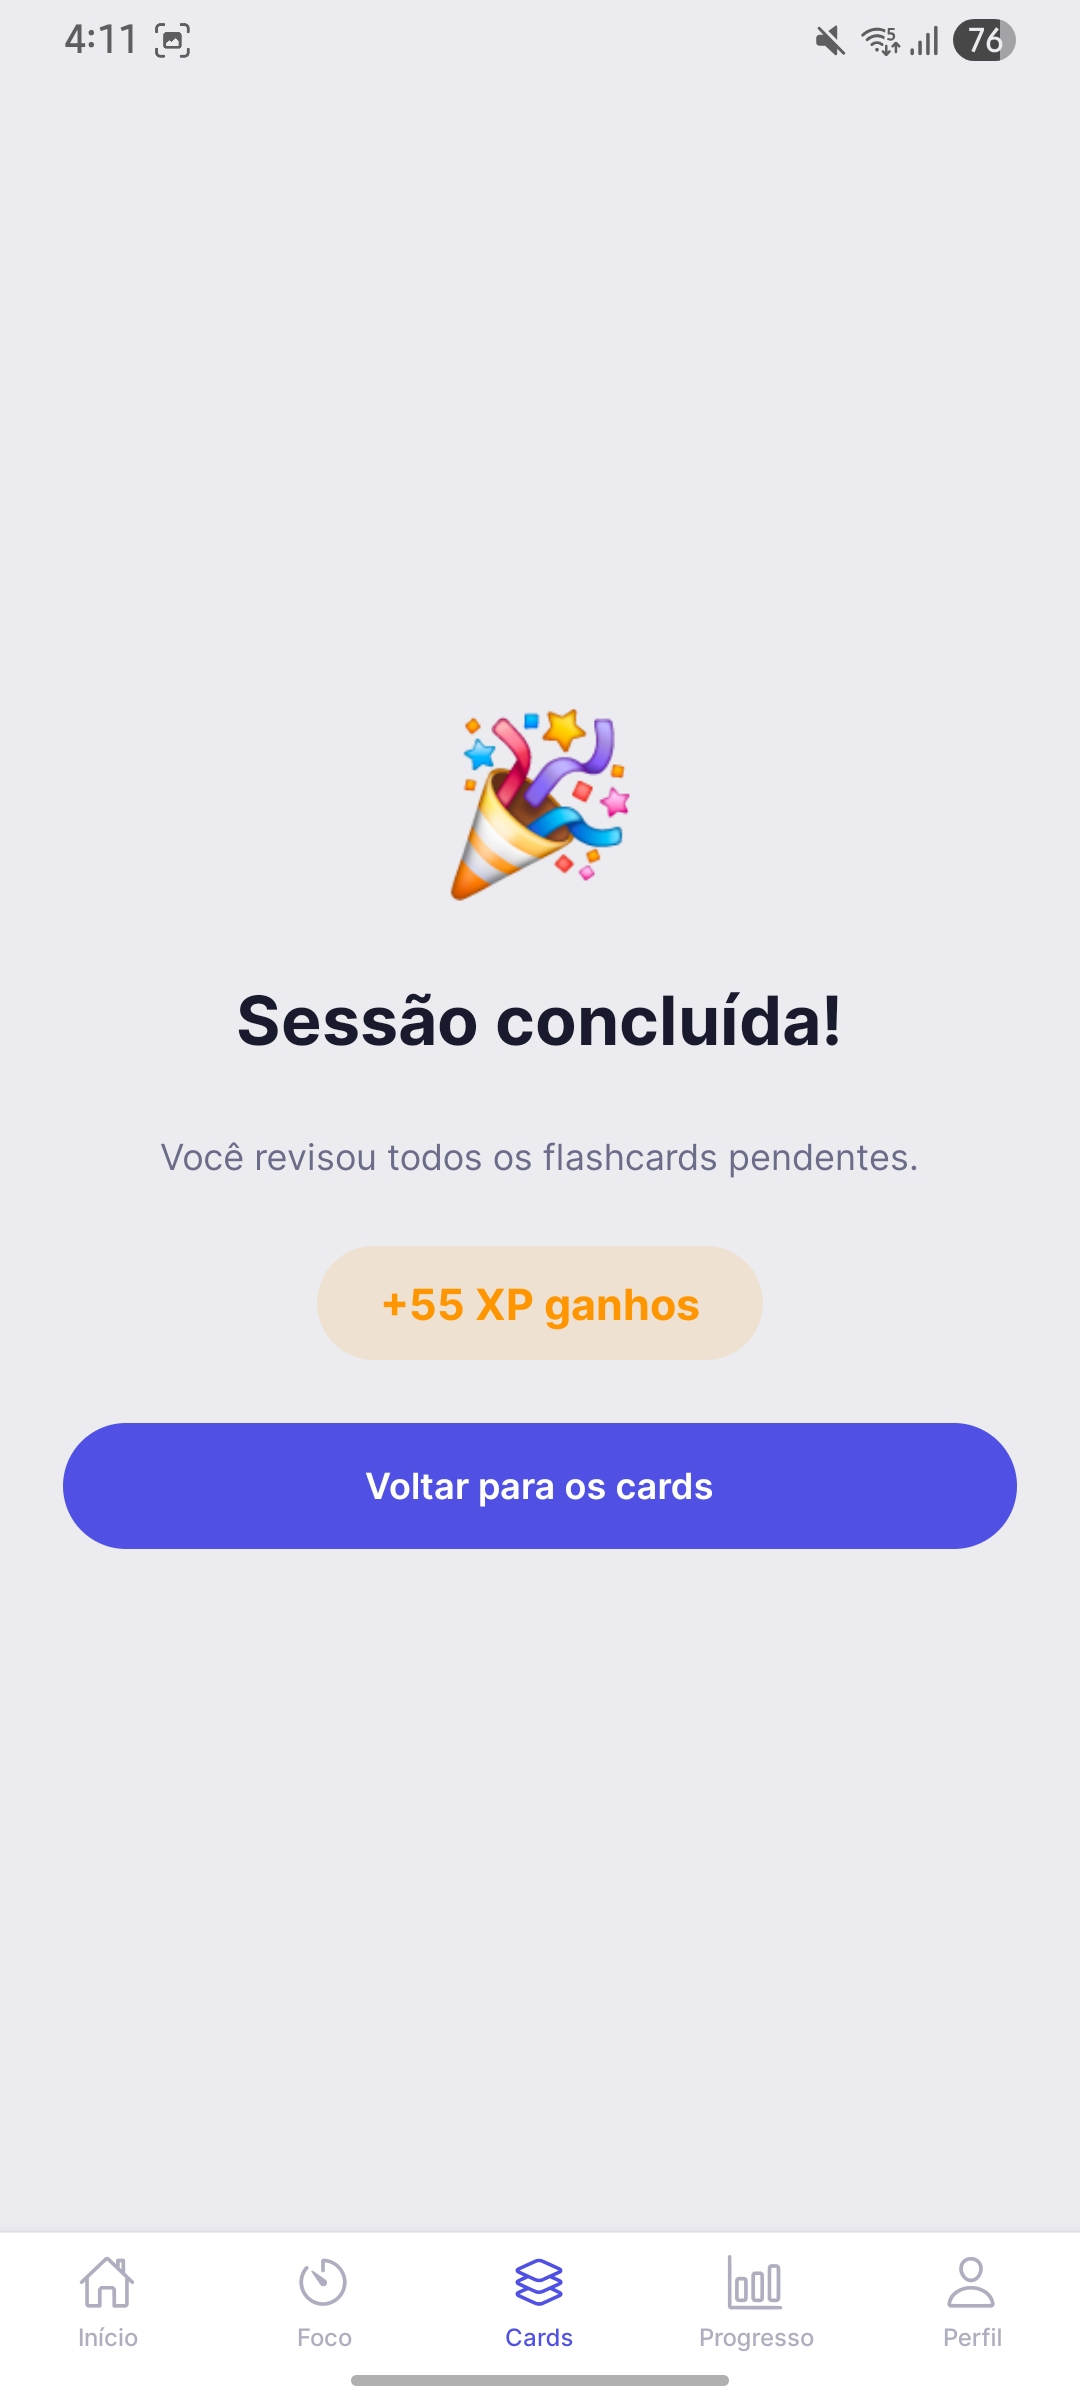
\includegraphics[height=0.7\textheight]{Imagens/PrototipoFigma/14_session_done.jpg}
    \par
    Fonte: autoria própria.
    \par
    \label{p15}
\end{figure}

\begin{figure}[H]
    \centering
    \caption{Tela de Progresso.}
    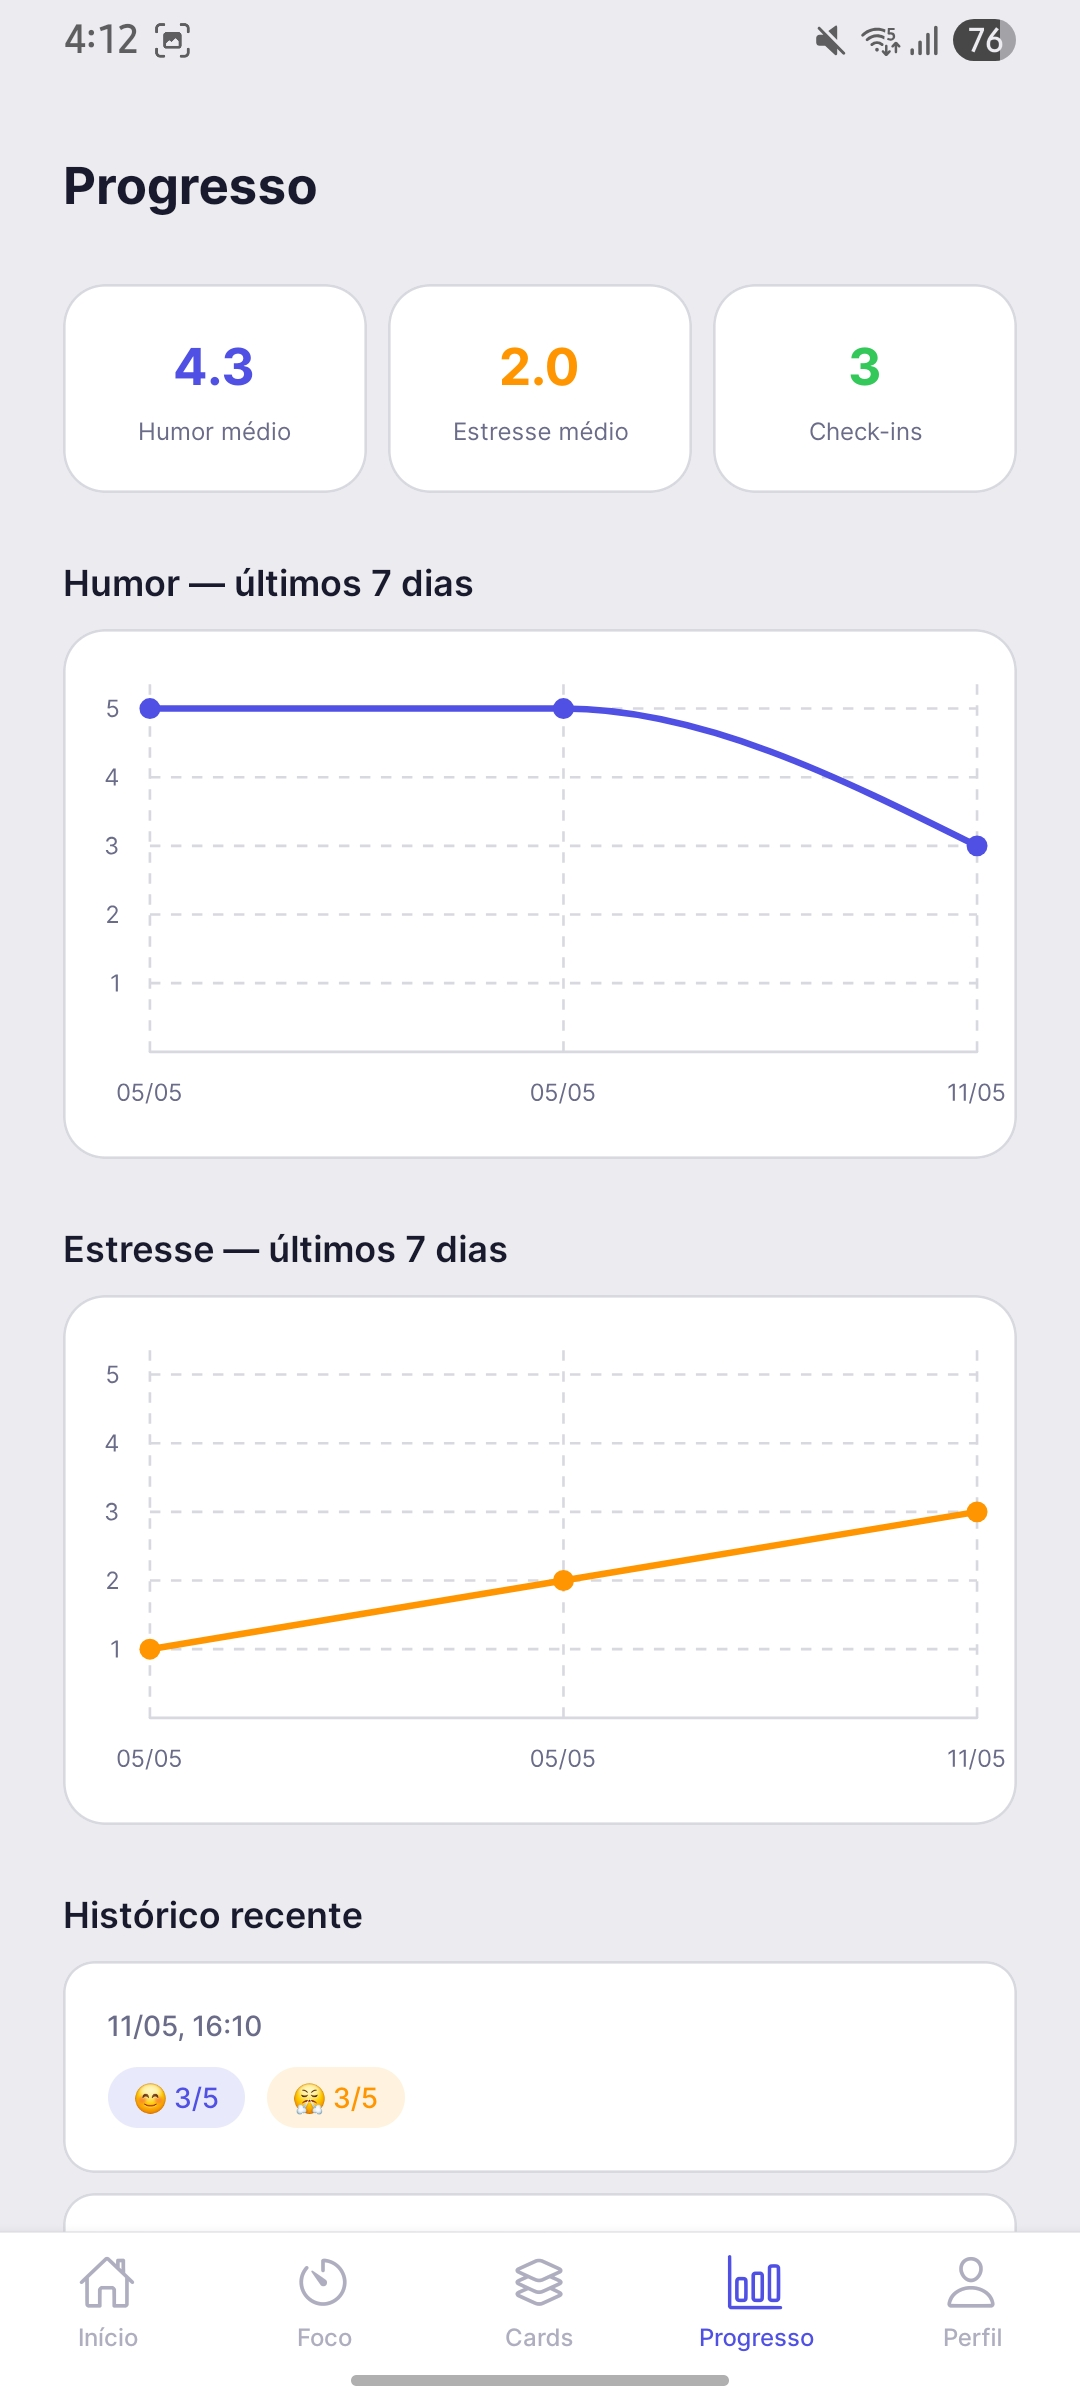
\includegraphics[height=0.7\textheight]{Imagens/PrototipoFigma/15_progresso.jpg}
    \par
    Fonte: autoria própria.
    \par
    \label{p16}
\end{figure}

\begin{figure}[H]
    \centering
    \caption{Tela de Perfil.}
    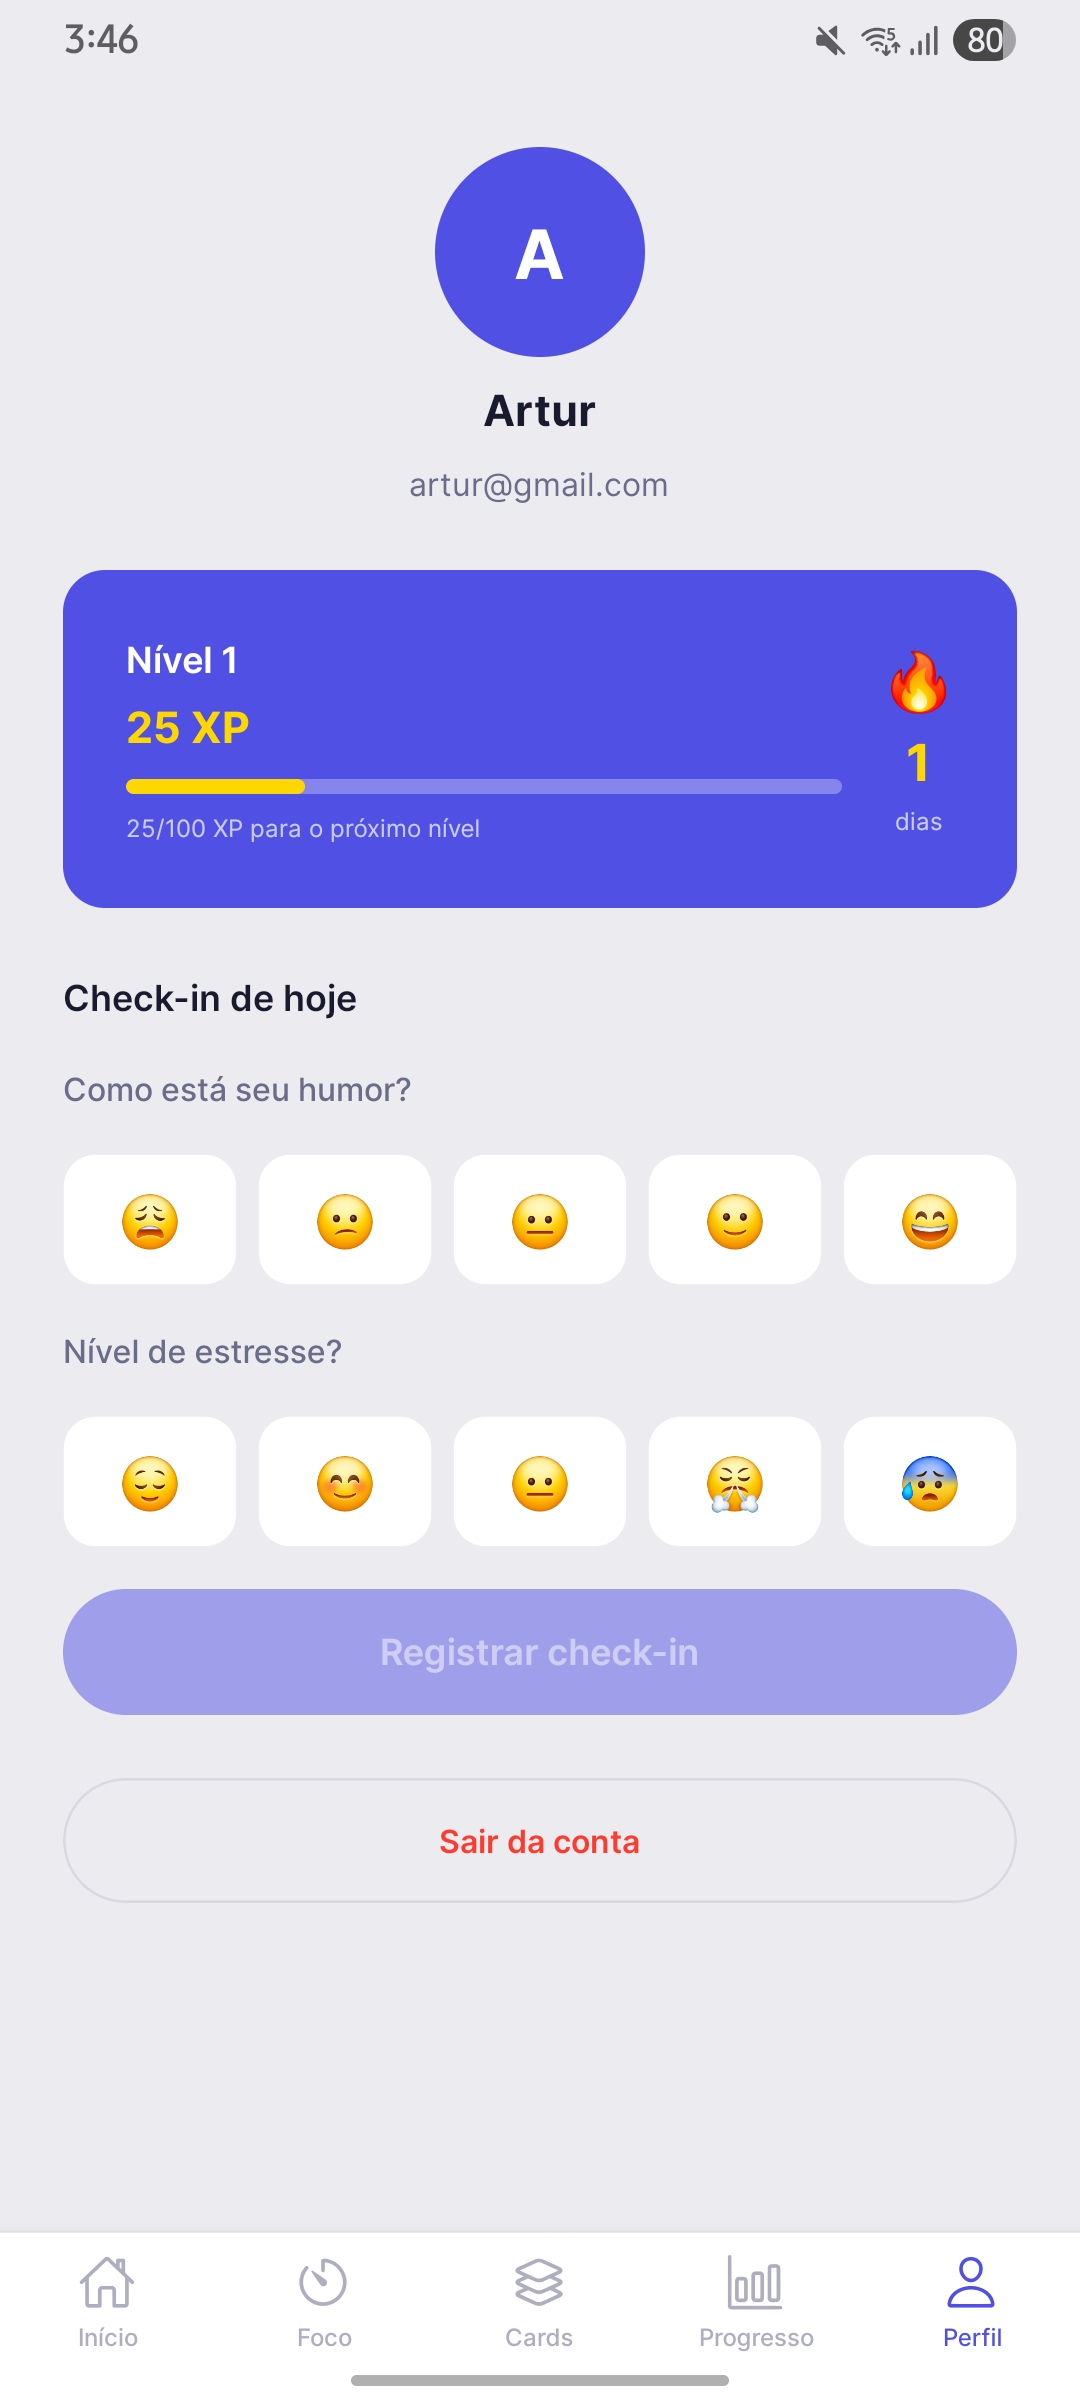
\includegraphics[height=0.7\textheight]{Imagens/PrototipoFigma/16_user.jpg}
    \par
    Fonte: autoria própria.
    \par
    \label{p17}
\end{figure}

\begin{figure}[H]
    \centering
    \caption{Tela de Perfil com Check-in Registrado.}
    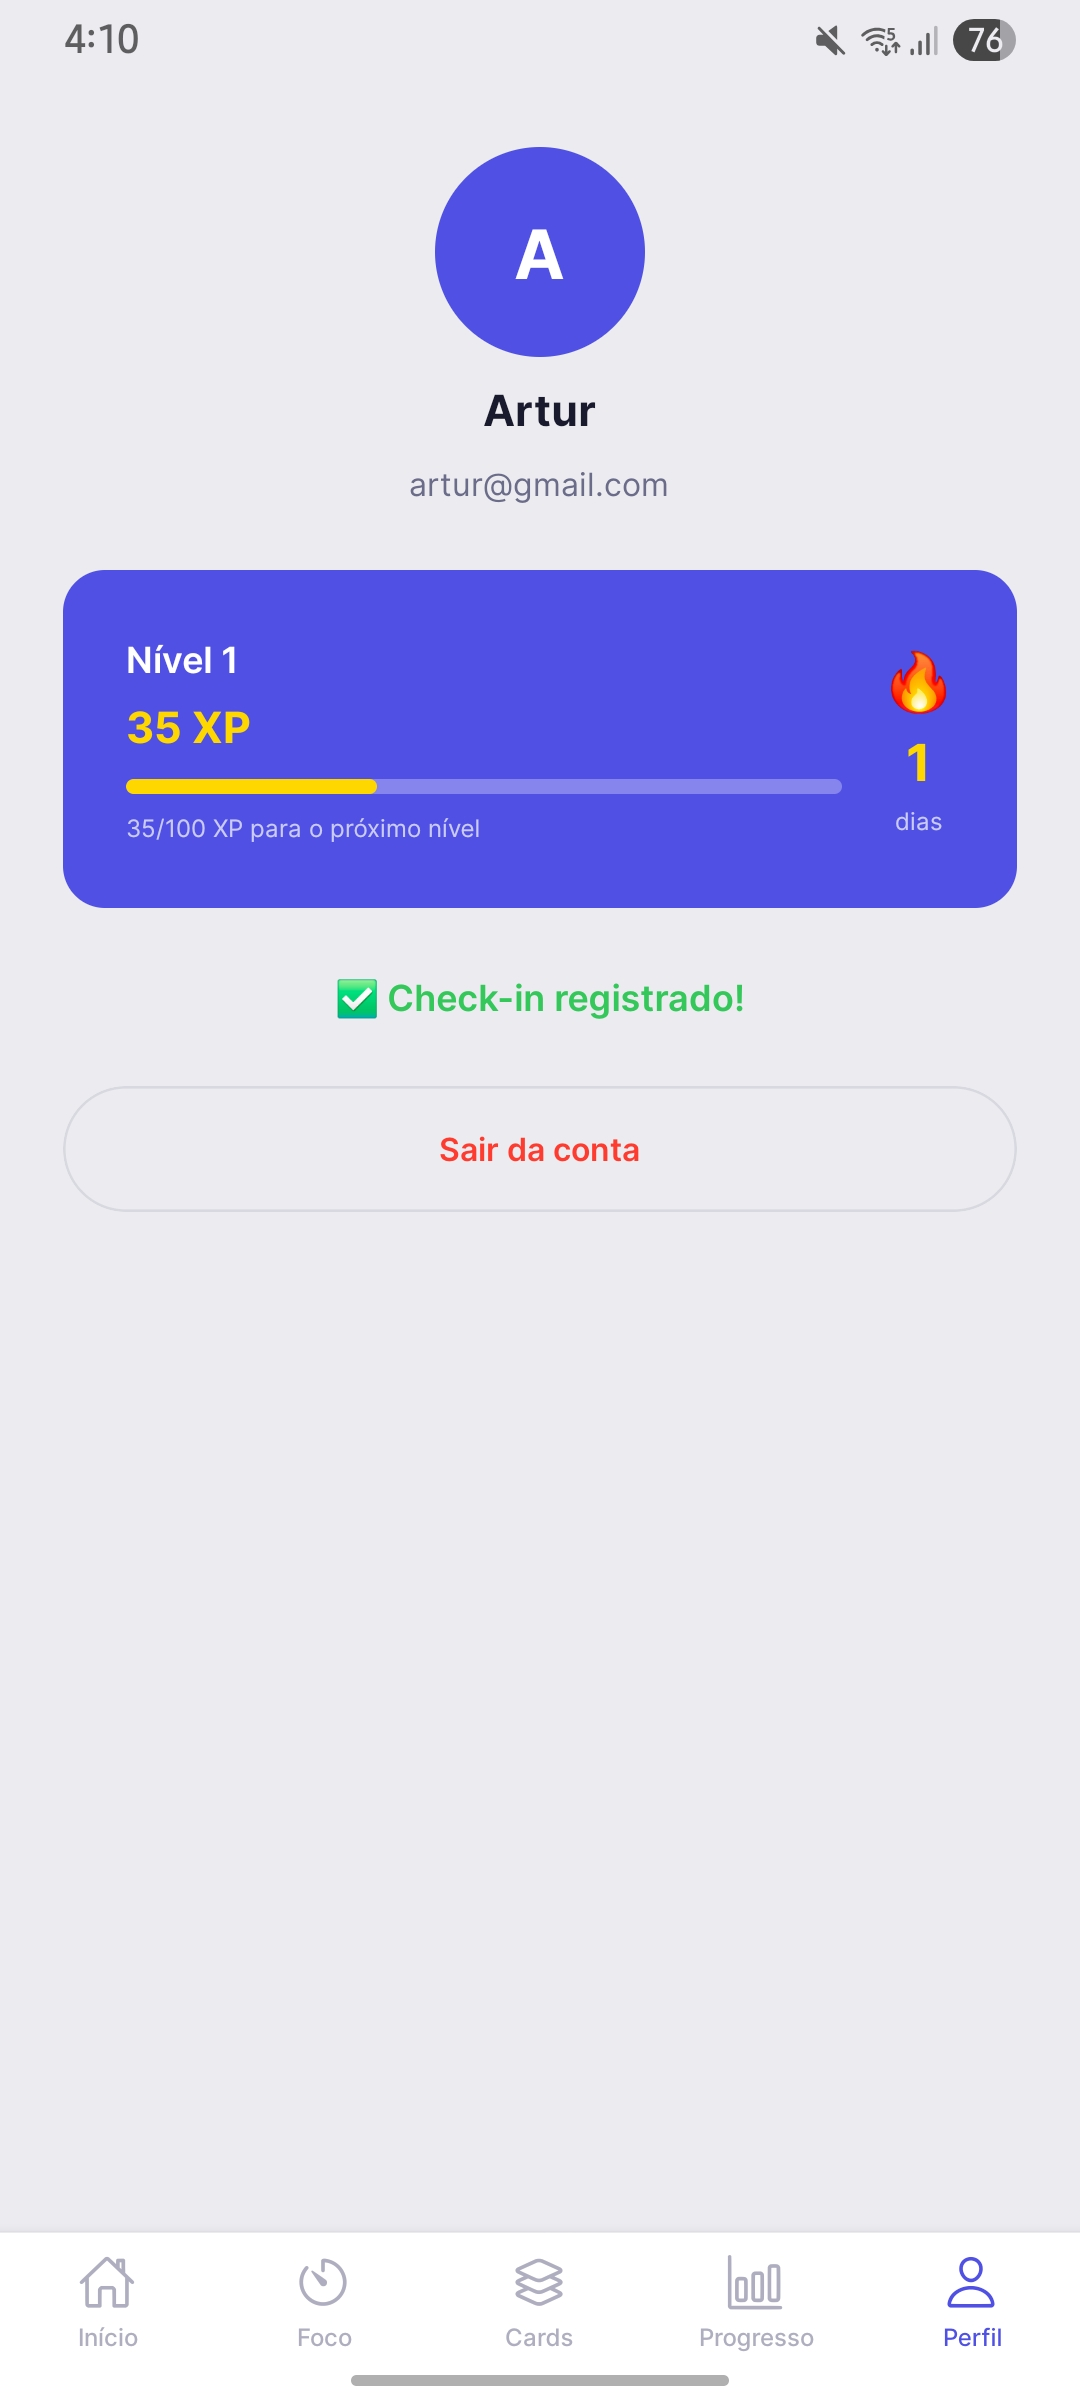
\includegraphics[height=0.7\textheight]{Imagens/PrototipoFigma/17_user_checkin.jpg}
    \par
    Fonte: autoria própria.
    \par
    \label{p18}
\end{figure}

\end{apendicesenv}
